% !TeX spellcheck = sr_SR-Serbian
% Format teze zasnovan je na paketu memoir
% http://tug.ctan.org/macros/latex/contrib/memoir/memman.pdf ili
% http://texdoc.net/texmf-dist/doc/latex/memoir/memman.pdf
% 
% Prilikom zadavanja klase memoir, navedenim opcijama se podešava 
% veličina slova (12pt) i jednostrano štampanje (oneside).
% Ove parametre možete menjati samo ako pravite nezvanične verzije
% mastera za privatnu upotrebu (na primer, u b5 varijanti ima smisla 
% smanjiti 

\documentclass[12pt,oneside]{memoir}

% Paket koji definiše sve specifičnosti mastera Matematičkog fakulteta
\usepackage{matfmaster}
%
% Podrazumevano pismo je ćirilica.
%   Ako koristite pdflatex, a ne xetex, sav latinički tekst na srpskom jeziku
%   treba biti okružen sa \lat{...} ili \begin{latinica}...\end{latinica}.
%
% Opicija [latinica]:
%   ako želite da pišete latiniciom, dodajte opciju "latinica" tj.
%   prethodni paket uključite pomoću: \usepackage[latinica]{matfmaster}.
%   Ako koristite pdflatex, a ne xetex, sav ćirilički tekst treba biti
%   okružen sa \cir{...} ili \begin{cirilica}...\end{cirilica}.
%
% Opcija [biblatex]:
%   ako želite da koristite reference na više jezika i umesto paketa
%   bibtex da koristite BibLaTeX/Biber, dodajte opciju "biblatex" tj.
%   prethodni paket uključite pomoću: \usepackage[biblatex]{matfmaster}
%
% Opcija [b5paper]:
%   ako želite da napravite verziju teze u manjem (b5) formatu, navedite
%   opciju "b5paper", tj. prethodni paket uključite pomoću: 
%   \usepackage[b5paper]{matfmaster}. Tada ima smisla razmisliti o promeni
%   veličine slova (izmenom opcije 12pt na 11pt u \documentclass{memoir}).
%
% Naravno, opcije je moguće kombinovati.
% Npr. \usepackage[b5paper,biblatex]{matfmaster}

% Pomoćni paket koji generiše nasumičan tekst u kojem se javljaju sva slova
% azbuke (nema potrebe koristiti ovo u pravim disertacijama)
\usepackage{pangrami}

% Paket koji obezbeđuje ispravni prikaz ćiriličkih italik slova kada
% se koristi pdflatex. Zakomentarisati ako na sistemu koji koristite ovaj
% paket nije dostupan ili ako ne radi ispravno.
\usepackage{cmsrb}
\usepackage{minted2}
\setminted{fontsize=\small}

% Ostali paketi koji se koriste u dokumentu
%\usepackage{listings} % listing programskog koda

% Datoteka sa literaturom u BibTex tj. BibLaTeX/Biber formatu
\bib{implementacija_tekst_editora_za_pisanje_koda}

% Ime kandidata na srpskom jeziku (u odabranom pismu)
\autor{Бојан Барџић}
% Naslov teze na srpskom jeziku (u odabranom pismu)
\naslov{Имплементација текст едитора за писање кода}
% Godina u kojoj je teza predana komisiji
\godina{2024}
% Ime i afilijacija mentora (u odabranom pismu)
\mentor{др Весна \textsc{Маринковић}, доцент\\ Универзитет у Београду, Математички факултет}
% Ime i afilijacija prvog člana komisije (u odabranom pismu)
\komisijaA{др Милан \textsc{Банковић}, доцент \\ Универзитет у Београду, Математички факултет}
% Ime i afilijacija drugog člana komisije (u odabranom pismu)
\komisijaB{др Иван \textsc{Чукић}, доцент\\ Универзитет у Београду, Математички факултет}
% Ime i afilijacija trećeg člana komisije (opciono)
% \komisijaC{}
% Ime i afilijacija četvrtog člana komisije (opciono)
% \komisijaD{}
% Datum odbrane (obrisati ili iskomentarisati narednu liniju ako datum odbrane nije poznat)
\datumodbrane{15. јануар 2016.}

% Apstrakt na srpskom jeziku (u odabranom pismu)
\apstr{%
\pangrami
}

% Ključne reči na srpskom jeziku (u odabranom pismu)
\kljucnereci{}

\begin{document}
% ==============================================================================
% Uvodni deo teze
\frontmatter
% ==============================================================================
% Naslovna strana
\naslovna
% Strana sa podacima o mentoru i članovima komisije
\komisija
% Strana sa posvetom (u odabranom pismu)
\posveta{}
% Strana sa podacima o disertaciji na srpskom jeziku
\apstrakt
% Sadržaj teze
\tableofcontents*

% ==============================================================================
% Glavni deo teze
\mainmatter
% ==============================================================================

% ------------------------------------------------------------------------------
\chapter{Увод}
% ------------------------------------------------------------------------------

\section{Текст едитори}

\paragraph{}
Текст едитор је програм за измену текстуалних датотека. Најчешћи типови датотека
који се измењују коришћењем ових програма су једноставне текстуалне датотеке, 
датотеке које садржe изворни код, код језика за означавање као и конфигурационе датотеке. 
Неки од најпознатијих оваквих програма су \begin{latinica}\textit{Visual Studio Code}
\end{latinica} \cite{VSC}, \begin{latinica}\textit{Notepad}\end{latinica} \cite{Notepad},
\begin{latinica}\textit{Notepad++}\end{latinica} \cite{Notepad++}, \begin{latinica}\textit{VIM}
\end{latinica} \cite{VIM} и \begin{latinica}\textit{Emacs}\end{latinica} \cite{Emacs}.

\paragraph{}
Постоји више врста текст едитора. Постоје едитори једноставног текста, где информација
о датотеци предсавља само текст. Док такође постоје и едитори богатог текста, где
информација о датотеци поред текста садржи и неке додатне информације везано за изглед
текста (фонт, величина фонта, боја текста, маргине). Овај рад ће се бавити искључиво
едиторима једноставног текста.

\chapter{Структуре података у текст едиторима}
\paragraph{}
Текст у датотеци се може посматрати као линеарни низ карактера, 
тако се и свака измена над тим текстом може посматрати као додавање текста у
неки део низа или брисање подниза текста. Када би комплетан садржај текстуалне датотеке
која је отворена чувана као јединствен низ карактера, операције уметања и брисања
текста биле би временски јако скупе (\(O(n)\), где је \(n\) дужина текста) и њихово узастопно
извршавање над неким великим текстом би имало за последицу изузетну неефикасност текст едитора.
Како би се овај проблем превазишао осмишљене су различите структуре података које ове операције
врше ефикасније. Најпознатије овакве структуре су бафер са размацима 
(енг. \begin{latinica}\textit{gap buffer}\end{latinica}), уже (енг. 
\begin{latinica}\textit{rope}\end{latinica}) и табела делова (енг. 
\begin{latinica}\textit{piece table}\end{latinica}).

\section{Бафер са размацима}
\paragraph{}
Бафер са размацима (енг. \begin{latinica}\textit{gap buffer}\end{latinica}) је структура
података која се заснива на идеји да постоји један линеаран низ чија је средина
"празна", док се са леве и десне стране налази текст. Како се врше измене над неким делом 
текста тако се средина "помера" превлачењем последњег елемента леве стране на почетак десне
или обрнуто. Када се бафер попуни (размак није довољно велики за нову операцију), тада се 
алоцира нови бафер већих димензија, најчешће дупло већи, и у њега се копира текст из старог
бафера.
\paragraph{}
У односу на класичан низ карактера, бафер са размацима је доста 
ефикаснији јер не захтева реалокацију низа при свакој измени. Ефикасност операција уметања и 
брисања зависи највише од тога колики је размак између индекса на коме се  
врши измена текста и леве или десне границе размака. Ако је размак већ на потребној позицији, 
временска сложеност је \(O(1)\). Међутим, ако је размак на једном крају а потребно је да 
се мења други крај текста сложеност ће бити \(O(n)\). У просечном случају временска 
сложеност наведених операција је константна, јер су карактери најчешће писани један за другим. 
Треба напоменути и то да је с времена на време потребно вршити реалокацију низа, 
која је линеарне сложености.

\paragraph{}
Разматрана структура података је једноставна за имплементацију и често се користи за једноставне
текстуалне уносе. Познати текст едитор \begin{latinica}\textit{Emacs}\end{latinica} \cite{Emacs} 
користи ову структуру у својој имплементацији. На слици \ref{fig:gap_buffer} приказана је 
илустрација рада бафера.

\begin{figure}[!ht]
  \centering
  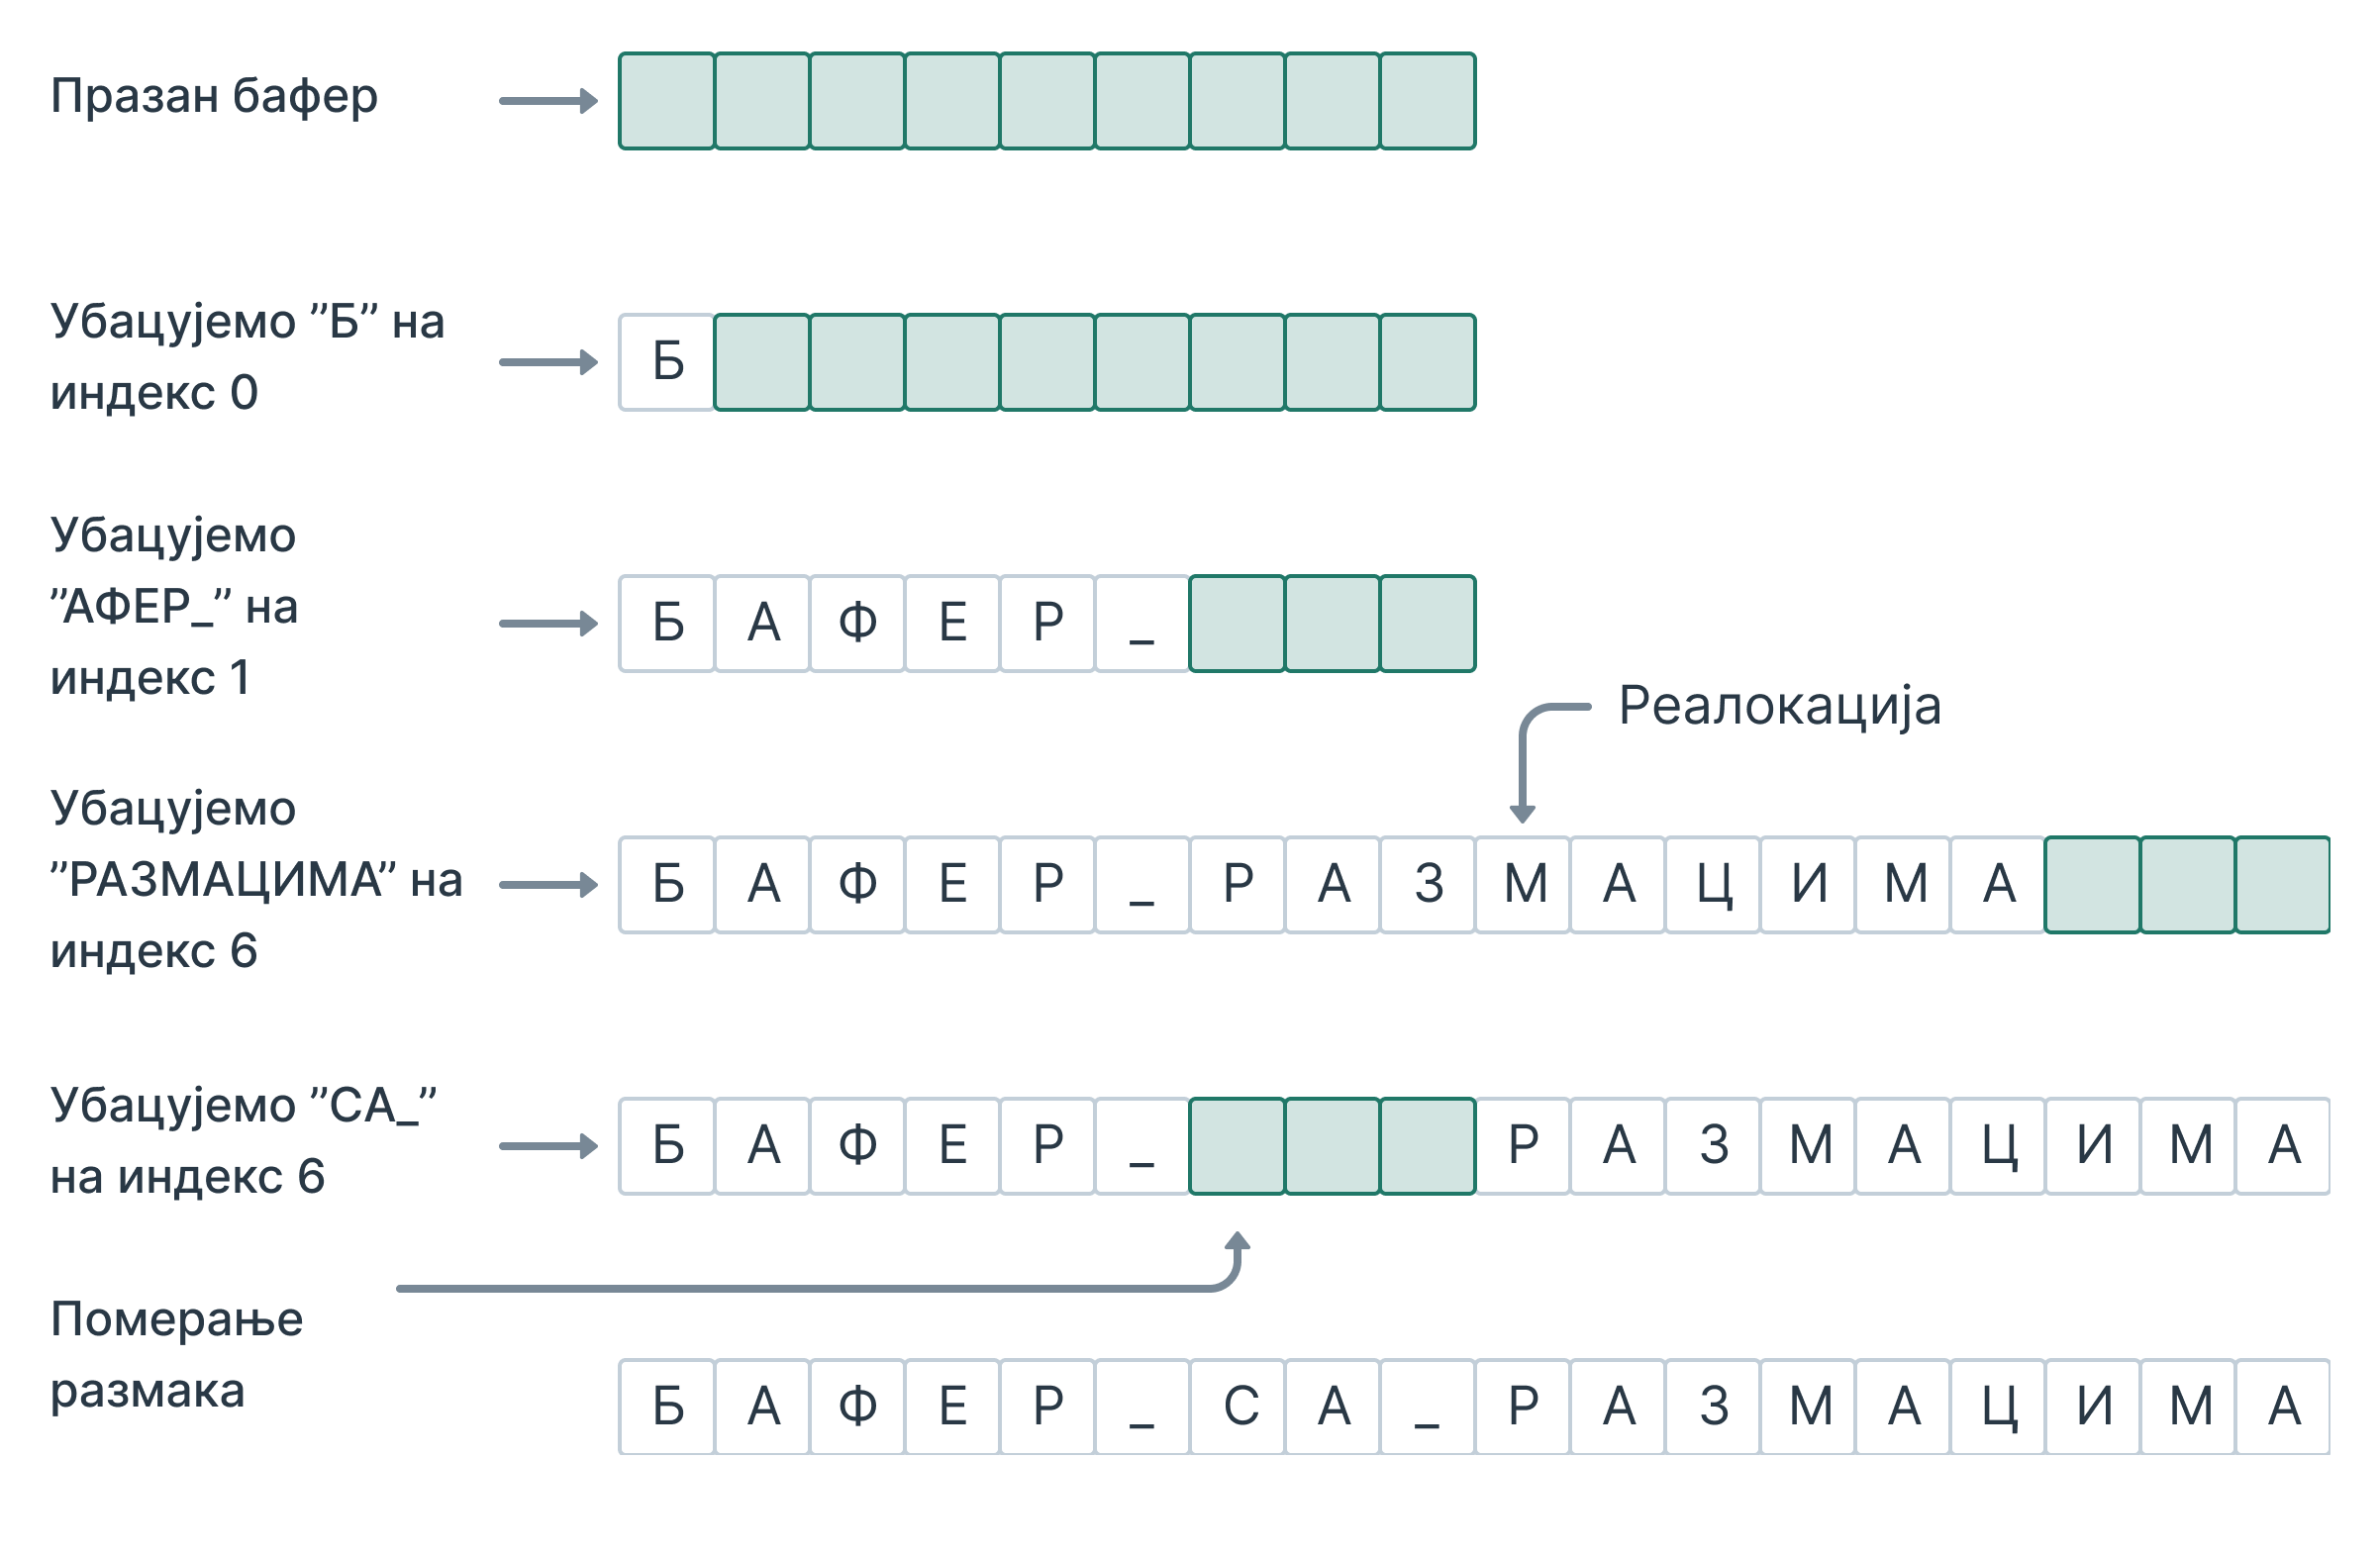
\includegraphics[width=1.1\textwidth]{images/Bafer_3.png}
  \caption{Илустрација бафера са размаком}
  \label{fig:gap_buffer}
\end{figure}

\paragraph{}
У првом кораку бафер је празан. У следећем кораку се додаје ниска \begin{latinica}\textit{"g"}\end{latinica} на почетну позицију. После тога на крај текста
се додаје ниска \begin{latinica}\textit{"ap\_"}\end{latinica}, а затим и ниска
\begin{latinica}\textit{"buffer"}\end{latinica}. У последњем кораку се додаје ниска
\begin{latinica}\textit{"between"}\end{latinica} на индекс број 6. Пошто је бафер  
у том тренутку пун, врши се реалокација. Када се текст прекопира у нови низ, 
помера се почетак празног дела на жељени индекс и додаје се нова ниска.

\section{Уже}
\paragraph{}
Уже (енг. \begin{latinica}\textit{rope}\end{latinica}) је бинарно стабло у коме сви чворови који нису
листови садрже број карактера у левом подстаблу тог чвора. У листовима се налазе ниске које 
садрже делове текста. Када се прође кроз листове од првог листа слева, добија се целокупан
текст.

\paragraph{}
Предност ове структуре у односу на обичну ниску је што операције као што су уметање, брисање
и претрага текста у просечном случају захтевају \(O(\log{}n)\) време (где је \(n\) дужина текста), 
а не \(O(n)\). Такође, није потребно чувати текст у непрекидном делу меморије, већ се чворови могу налазити на одвојеним местима.

\paragraph{}
Мане ужета јесу што је то комплексна структура и чешће су грешке како у раду са њом, тако и при
њеној имплементацији. Поред тога, заузима више меморије него обична ниска 
(због родитељских чворова који повезују листове).

\subsection{Претрага}
\paragraph{}
Приступ карактеру на \(i\)-том  индексу се врши тако што се рекурзивно пролази кроз стабло 
почевши од корена. Ако је индекс мањи од вредности у текућем чвору, настављамо претрагу у његовом левом 
подстаблу. У супротном од \(i\) се одузима вредност у тренутном чвору и наставља се претрага у
његовом десном подстаблу. Када се наиђе на лист враћа се \(i\)-ти карактер из ниске која се налази
у чвору. Сложеност операције је иста као код претраге бинарног стабла, а то је \(O(\log{}n)\).
Пример претраге дат је на слици \ref{fig:rope_search}.

\begin{figure}
  \centering
  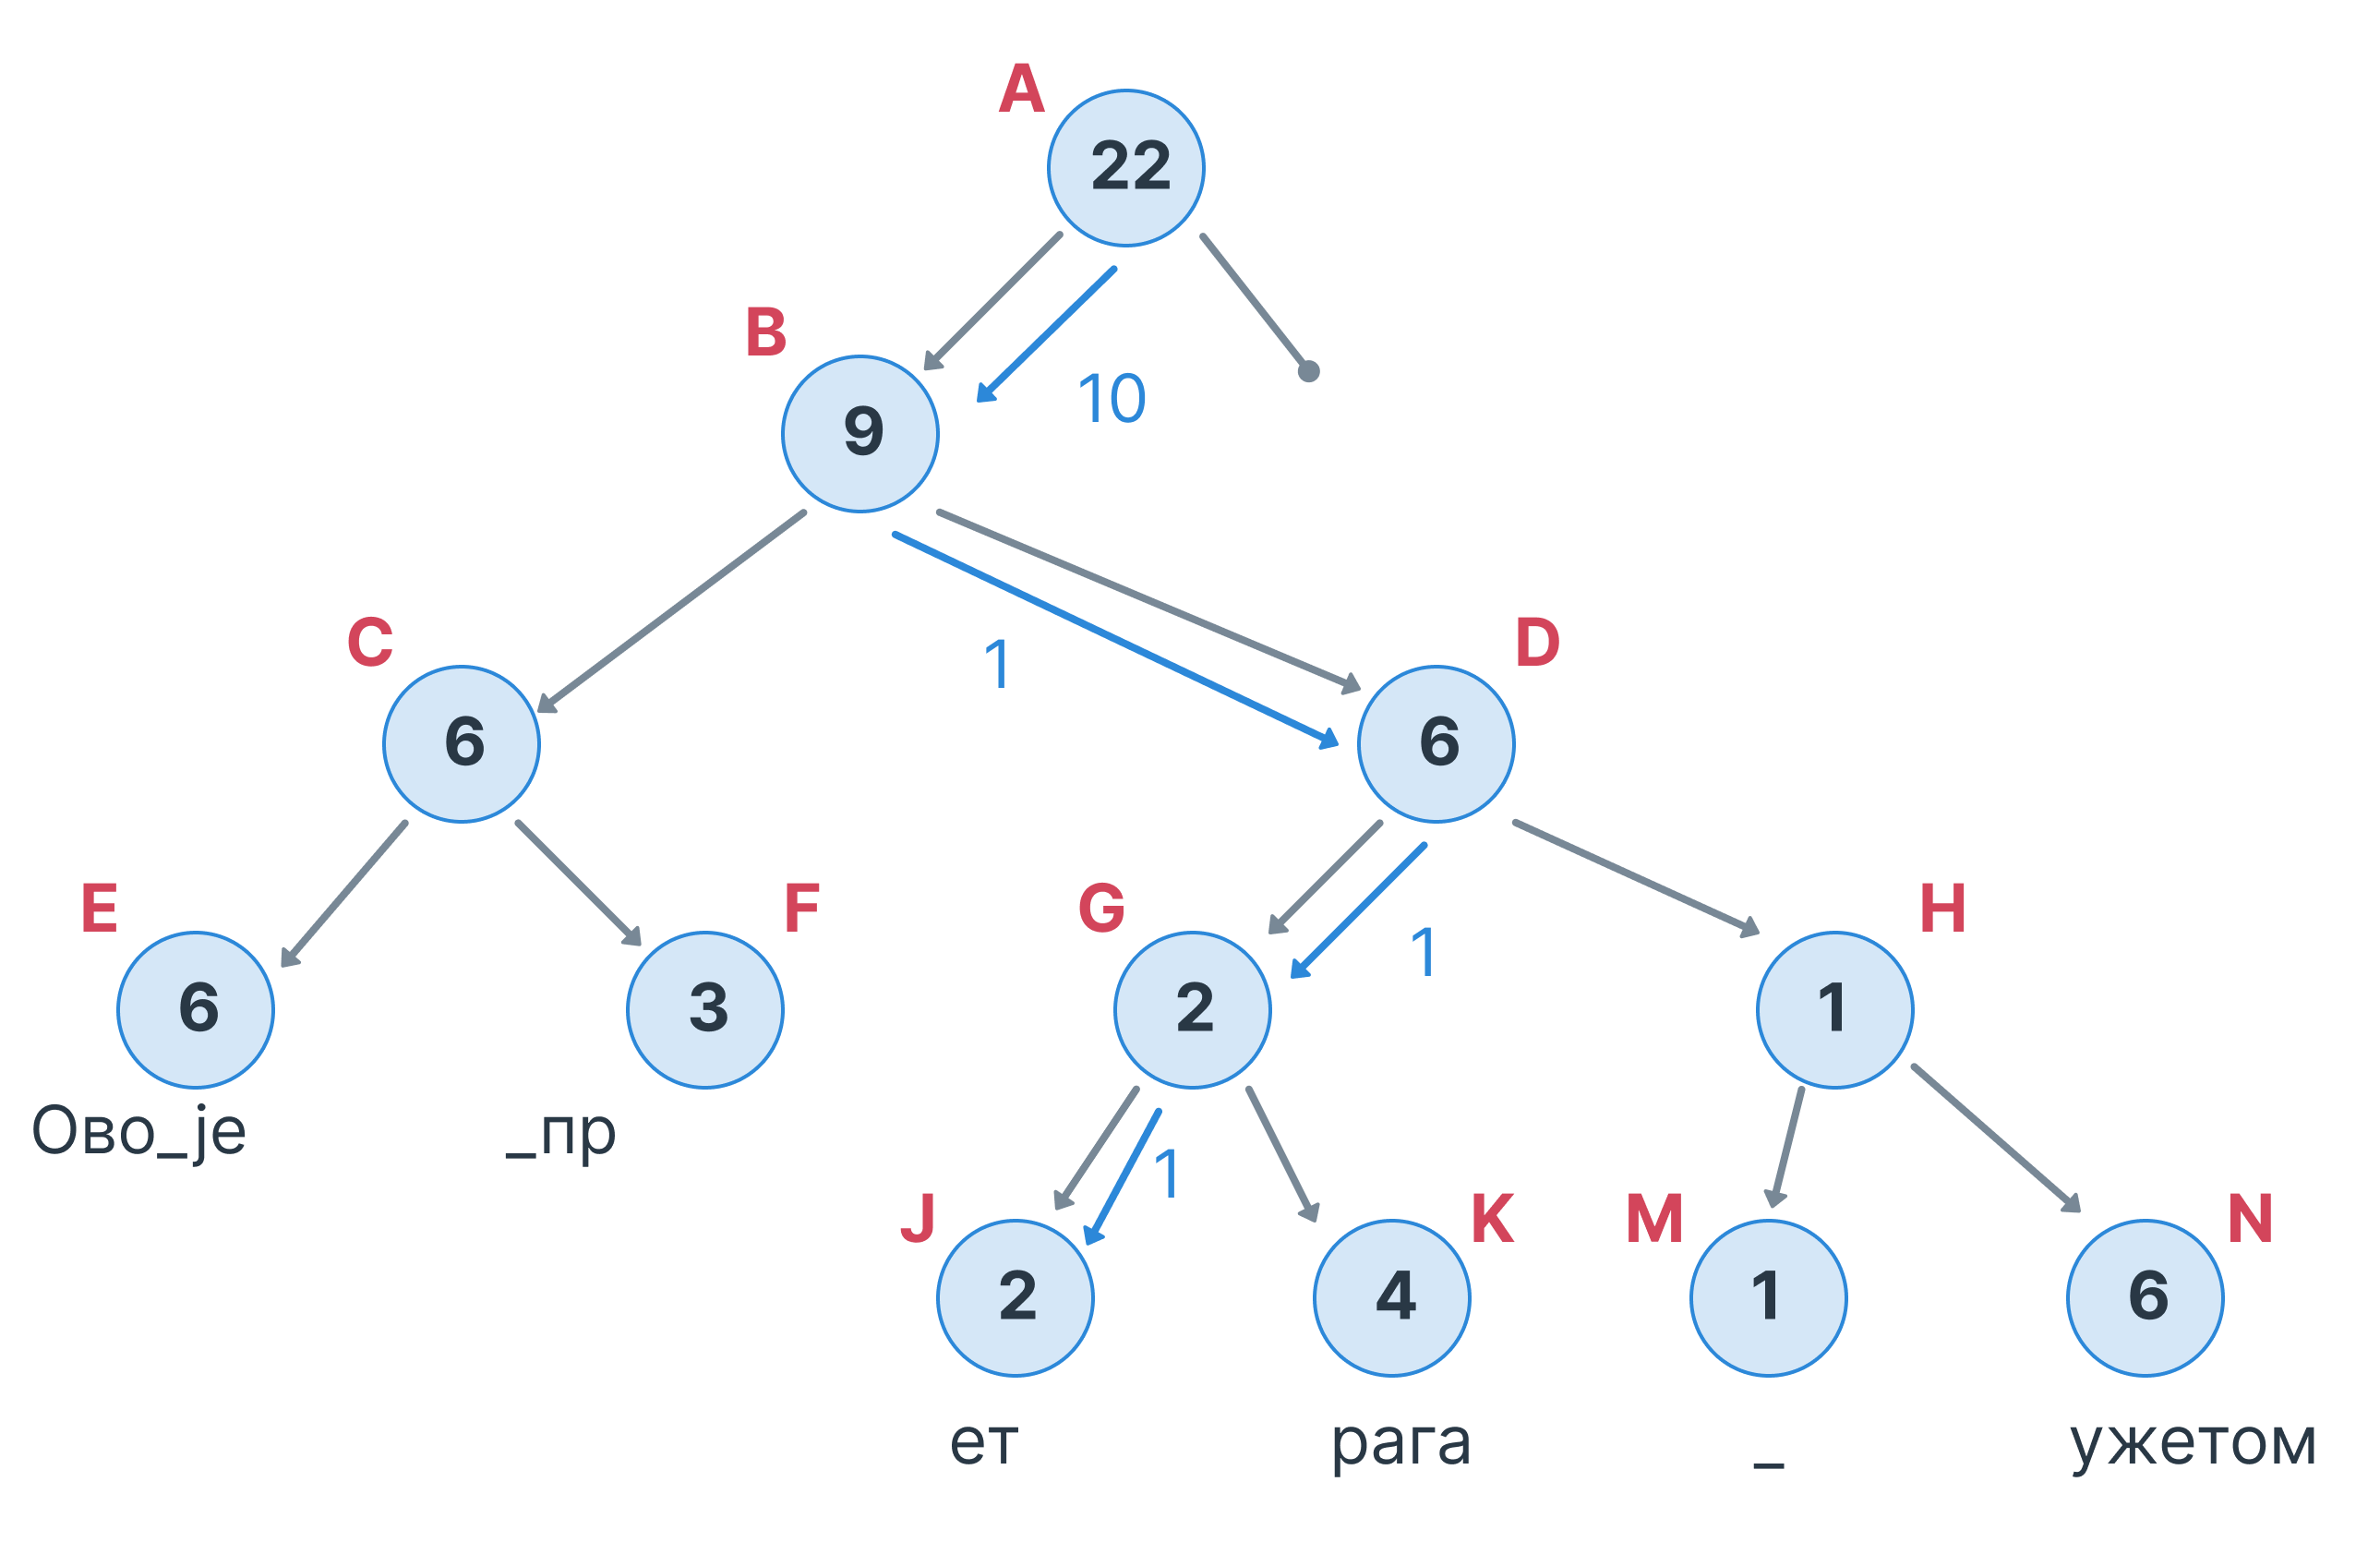
\includegraphics[width=0.8\textwidth]{images/rope_search_1.png}
  \caption{Претрага помоћу ужета}
  \label{fig:rope_search}
\end{figure}

\paragraph{}
Тражи се карактер на индексу број 10. Прво се обилази корен који садржи дужину укупног текста, 
пошто је тражени индекс мањи од вредности у тренутном чвору иде се у његово лево подстабло. Следећи чвор
садржи вредност 9, што значи да је тражени индекс већи од вредности. Одузима се та вредност од траженог
индекса и претрага се наставља у десном подстаблу тренутног чвора. Сада је тражени индекс 1 и он се
поново упоређује са тренутним чвором. Пошто је 1 мање од 6 прелази се у лево подстабло. 
У следећем чвору вредност је 2 па се поново иде у лево подстабло. 
На крају се наилази на лист и у нисци коју он садржи се дохвата карактер на индексу 1 
и прослеђује се као повратна вредност.

\paragraph{}
Пре него што буде обрађена операција брисања, прво ће бити уведене две нове операције које ће
бити потребне за њену реализацију. Прва операција је надовезивање једног ужета на друго,
док је друга операција дељење једног ужета на два нова ужета по неком карактеру.


\subsection{Конкатенација}
\paragraph{}
Конкатенација или надовезивање је операција којом се на уже, које садржи текст \(t_1\), 
надовезује друго уже које садржи текст \(t_2\) и добија се ново уже које садржи текст \(t_1t_2\).
Конкатенација два ужета, \(r_1\) и \(r_2\), се врши тако што се направи нови родитељски чвор
чије ће лево дете бити корен од \(r_1\), а десно корен од  \(r_2\). Вредност новог чвора ће
бити сума дужина ниски у свим листовима ужета \(r_1\). Да би израчунали вредност новог корена
потребно је израчунати суму дужина ниски свих листова који се налазе у \(r_1\). То се постиже
рекурзивним обиласком \(r_1\), где се на коначну суму додаје вредност тренутног чвора и
затим се рекурзивно обилази десно подстабло тренутног чвора. Сложеност ове 
операције је \(O(\log{}n)\) за балансирано стабло. Пример конкатенације два 
ужета се може видети на слици \ref{fig:rope_concat}

\begin{figure}
  \centering
  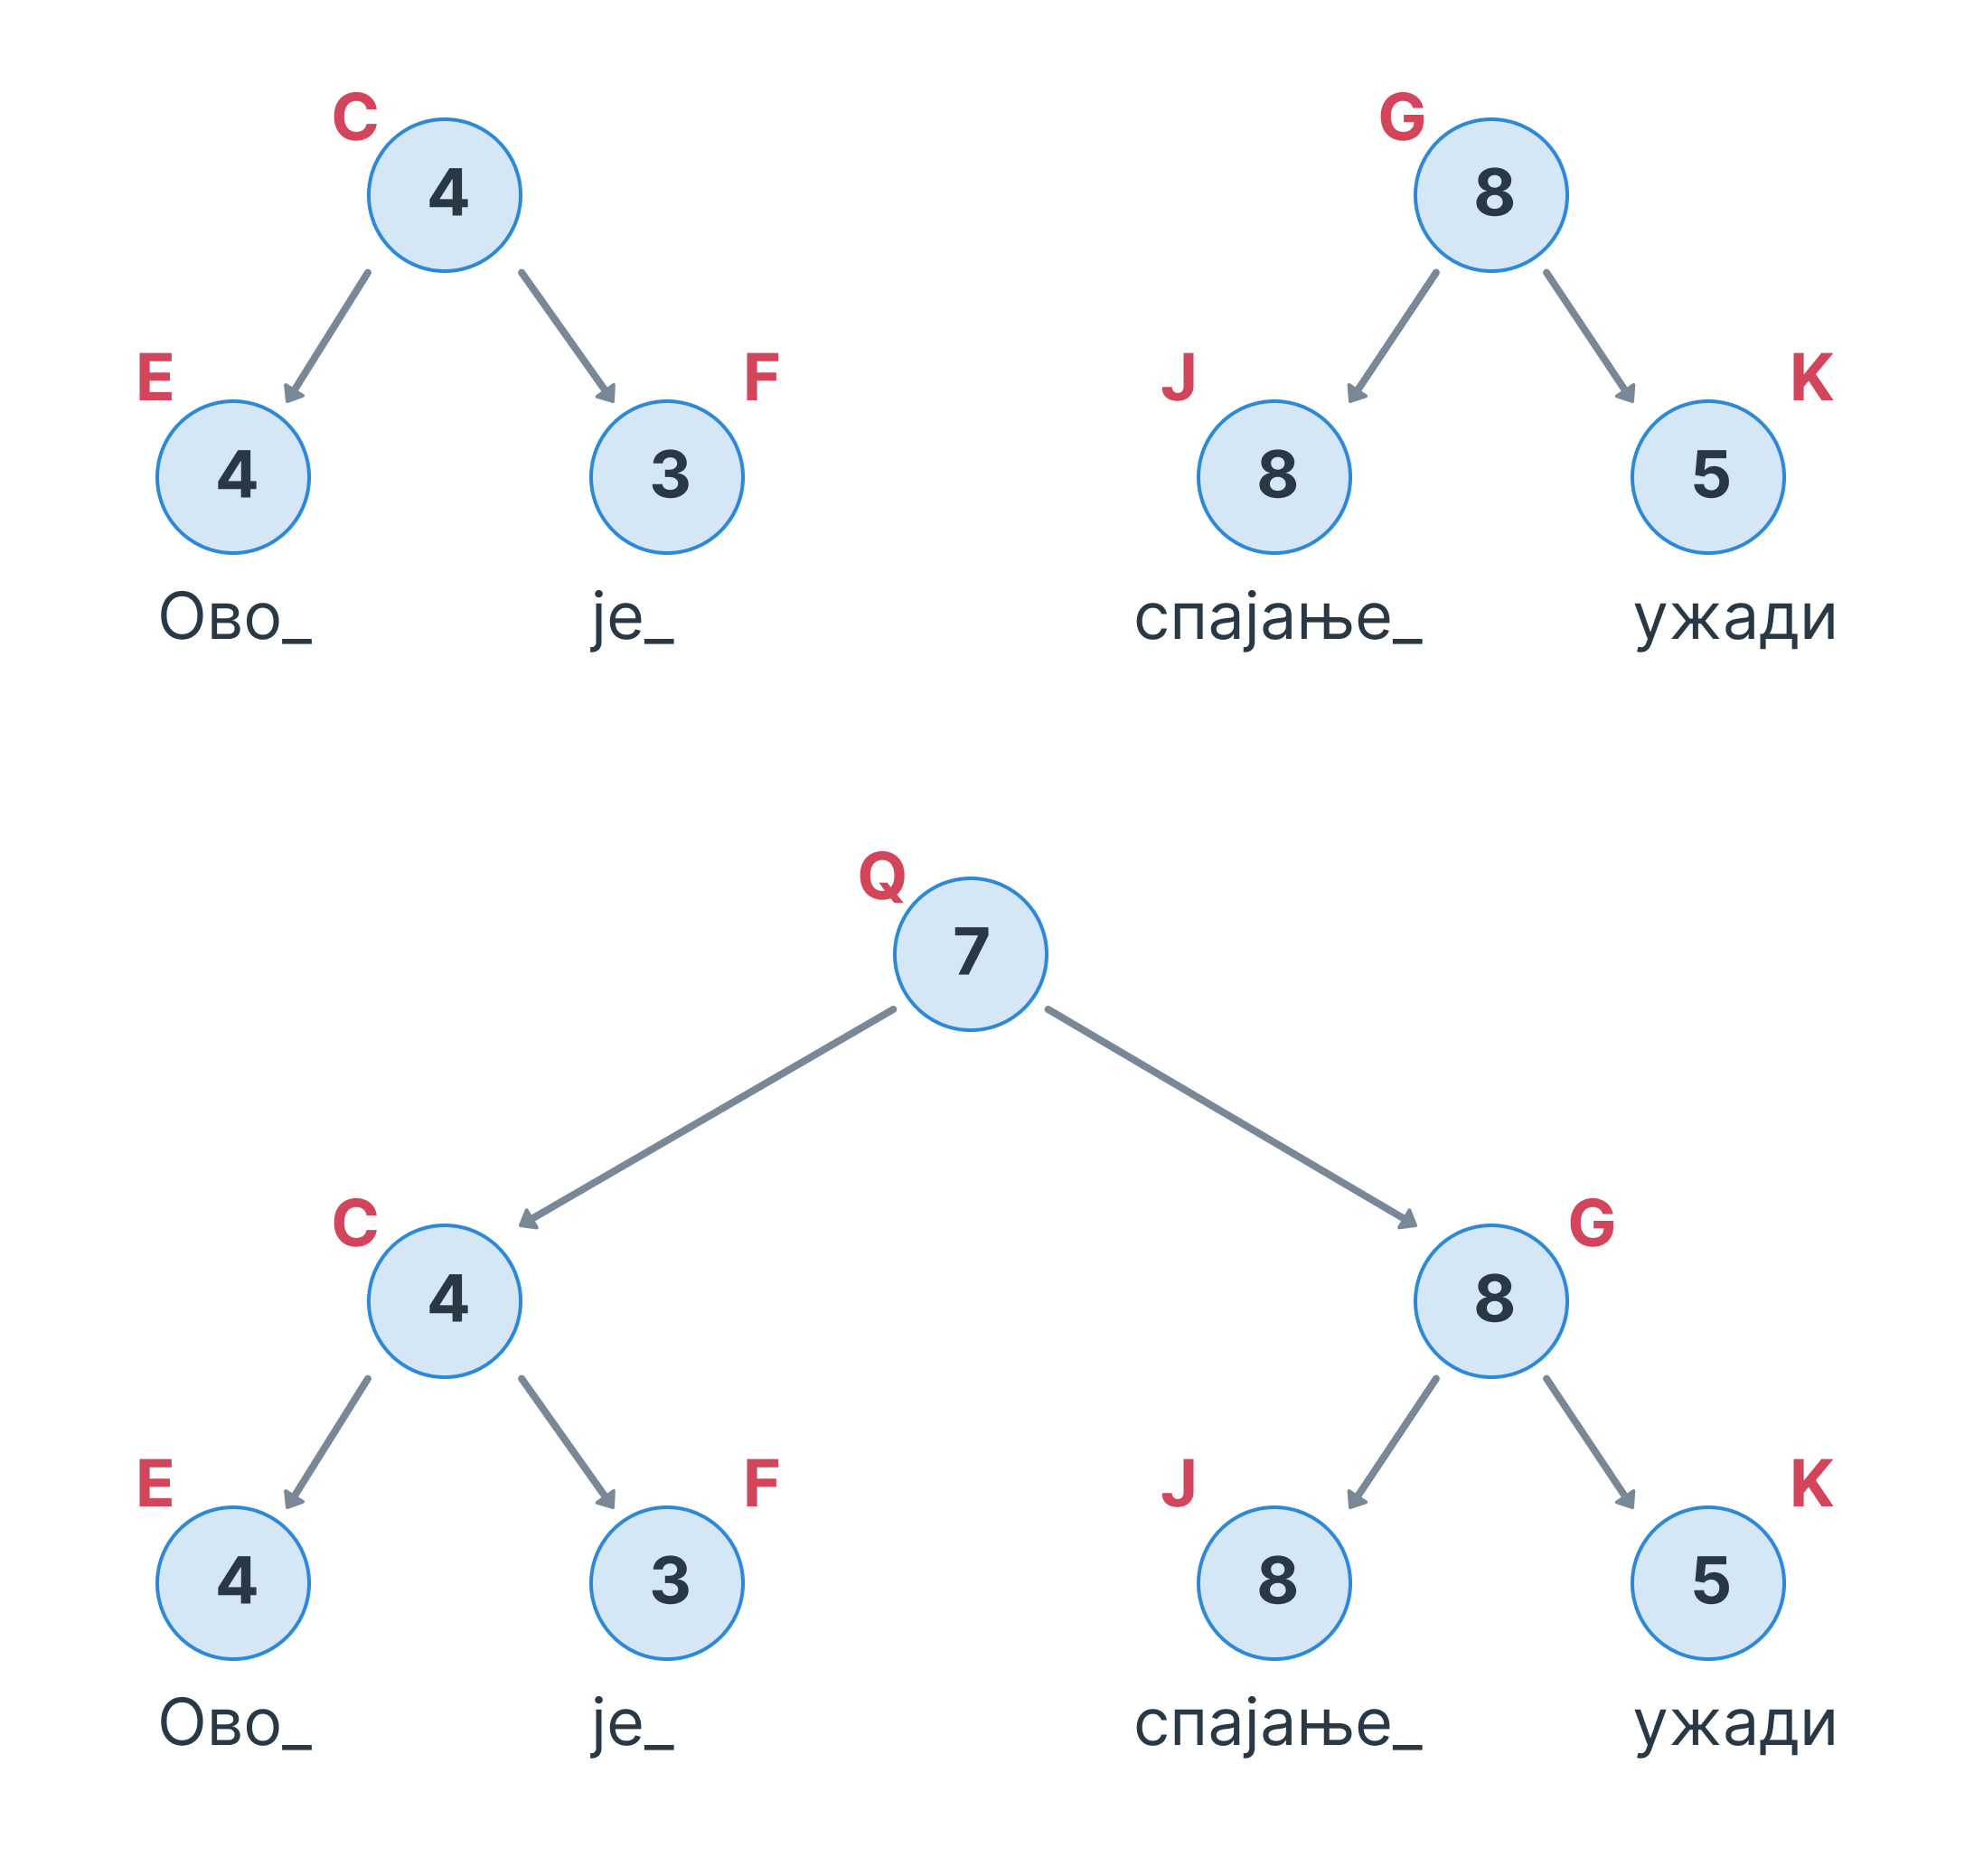
\includegraphics[width=0.8\textwidth]{images/rope_concat_1.png}
  \caption{Конкатенација два ужета}
  \label{fig:rope_concat}
\end{figure}

\subsection{Дељење}
\paragraph{}
Дељење ниске \(s\) по индексу \(i\) на две ниске, \(s_1\) и \(s_2\),
где \(s_1\) садржи карактере од почетка ниске \(s\) до \(i\)-тог индекса (укључујући и карактер на 
\(i\)-том индексу), а \(s_2\) садржи карактере десно од \(i\)-тог индекса па до краја ниске,
се врши на следећи начин.

\paragraph{}
Најпре се налази \(i\)-ти карактер, ако је то последњи карактер ниске у листу онда се не ради ништа.
У супротном се дели лист на два нова листа, где је \(i\)-ти карактер последњи карактер ниске
левог листа. Нека је лист чији је \(i\)-ти карактер последњи у нисци означен са \(d\). Сада
се листови деле у две групе \(l_1\) и \(l_2\). У \(l_1\) се налазе листови лево од \(d\) као и сам \(d\), док се у \(l_2\) налазе листови десно од \(d\). Листови из се \(l_2\) одвајају од 
главног ужета и затим се спајају заједно. Алгоритам се завршава тако што се балансирају 
два новодобијена ужета.

\paragraph{} 
Сложеност је иста као код претходних операција. На слици \ref{fig:ropе_split} се може видети пример
дељења. Дељење се врши по индексу 10. Прво се проналази карактер на датом индексу на начин описан
у делу о претрази. Затим се проверава да ли је тај карактер последњи у листу, пошто јесте,
врши се подела на \(l_1\) и \(l_2\) по том листу.

\begin{figure}
  \centering
  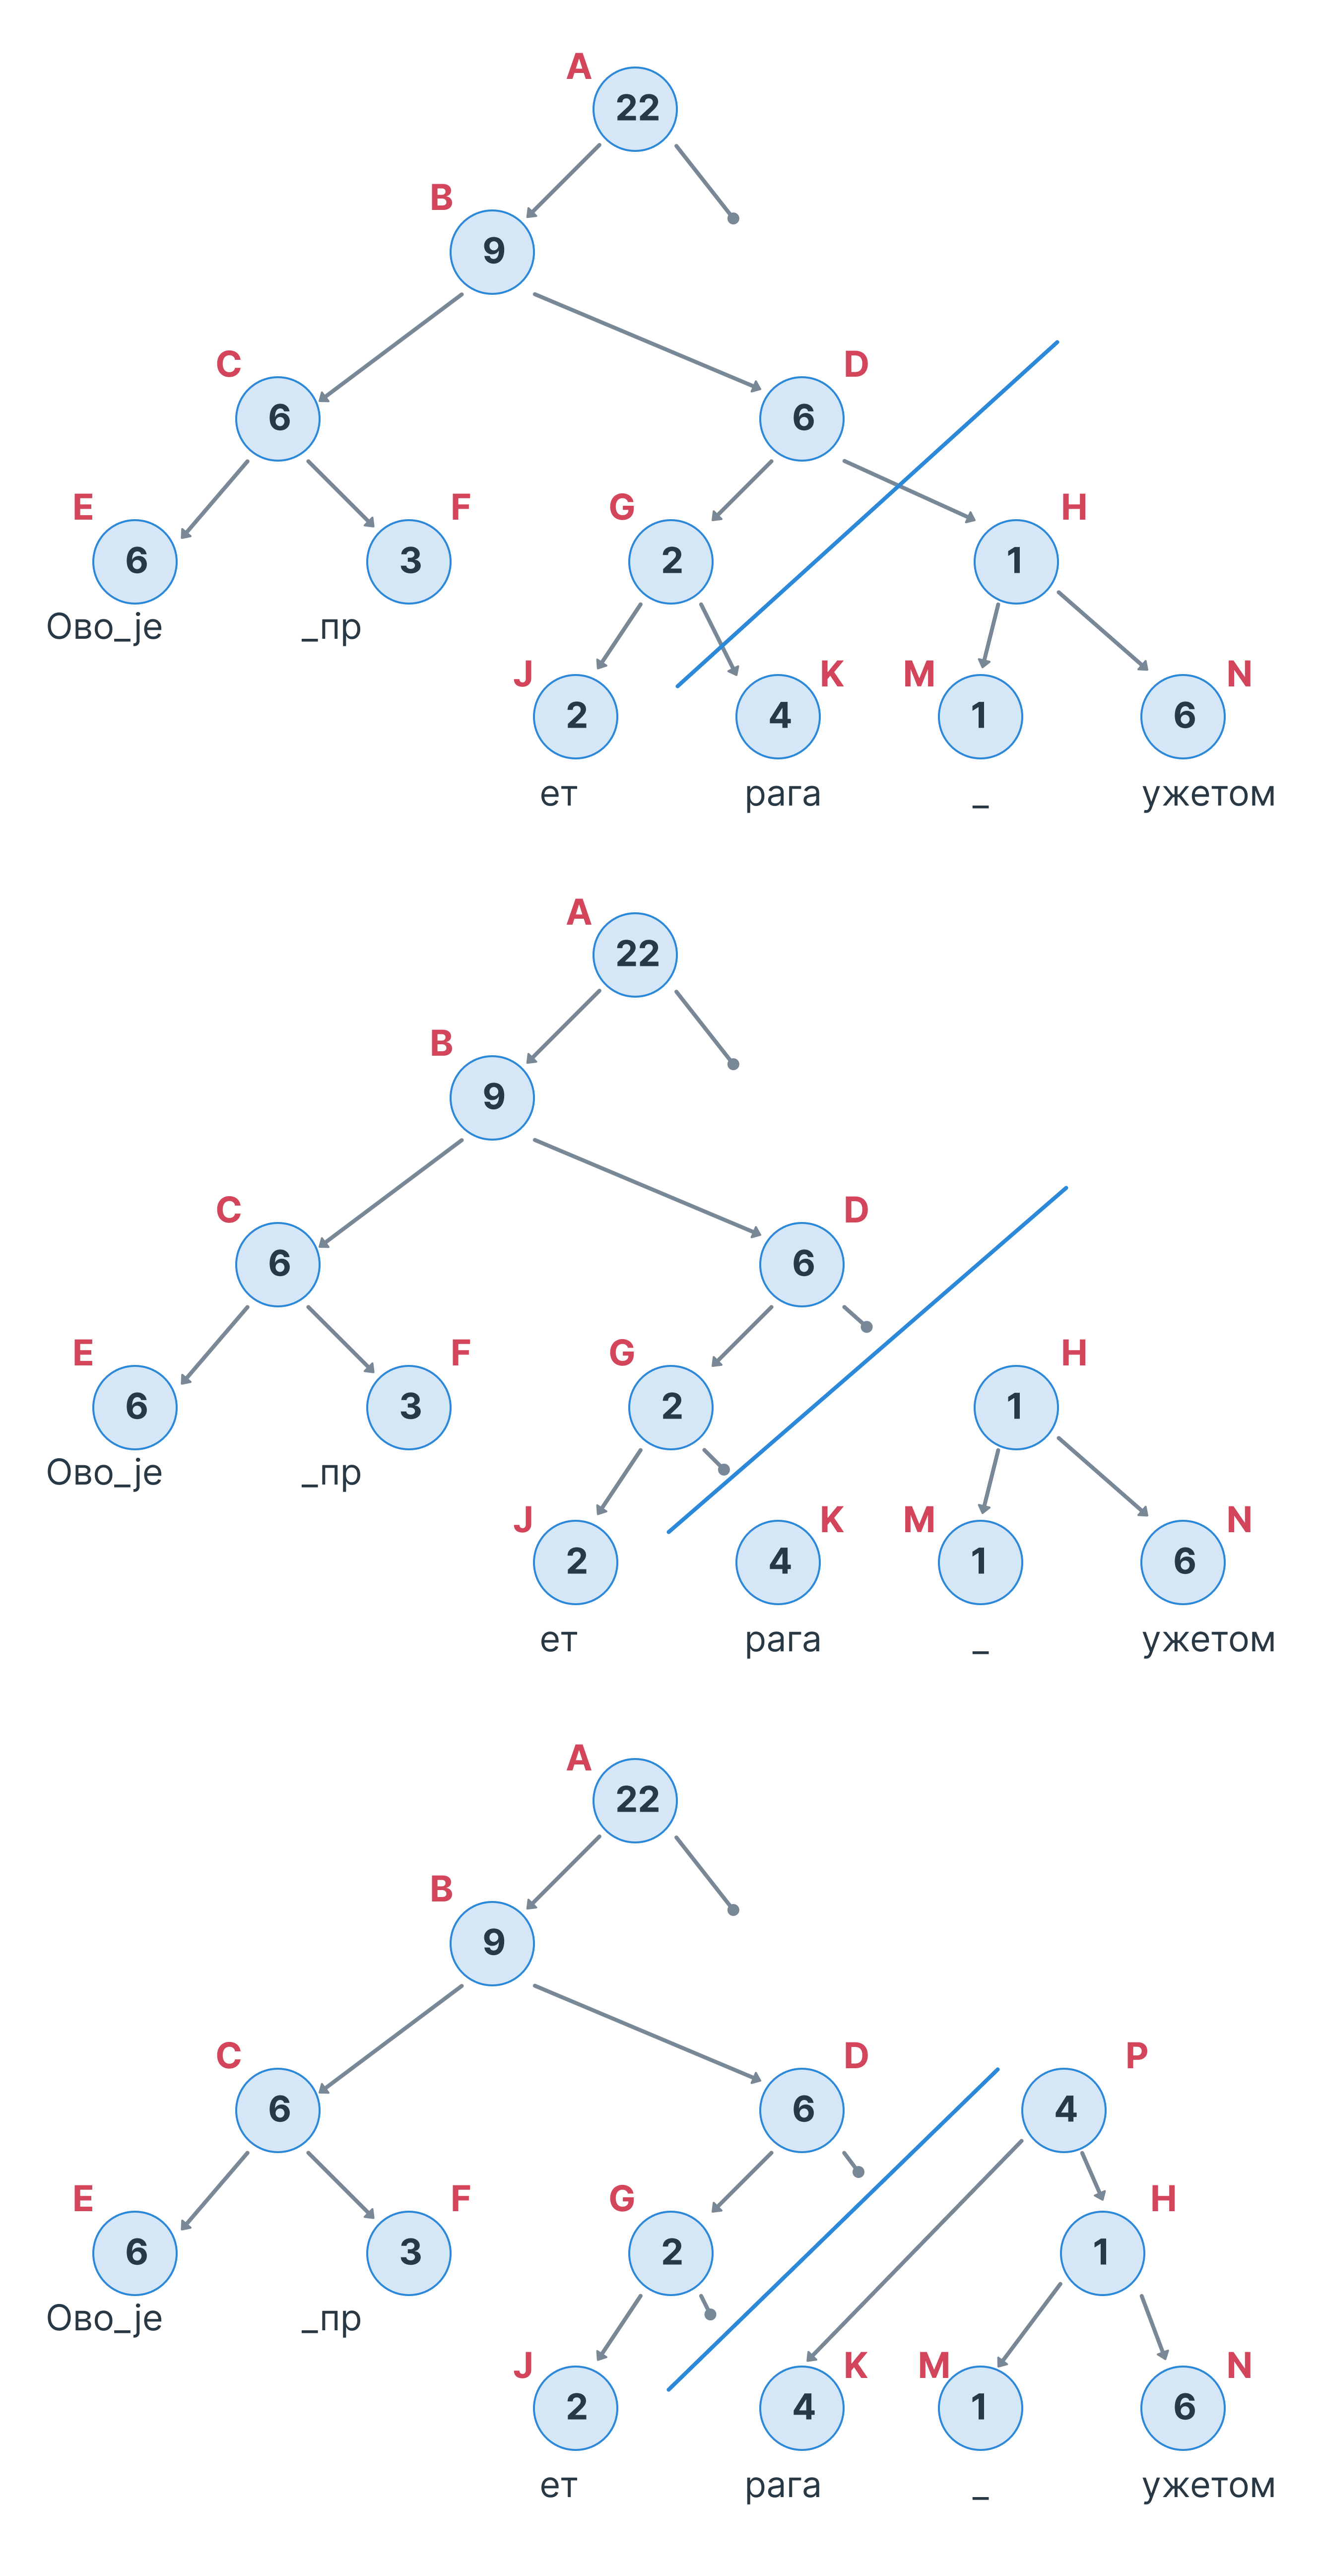
\includegraphics[width=0.8\textwidth]{images/rope_split_1.png}
  \caption{Дељење ужета}
  \label{fig:ropе_split}
\end{figure} 

\subsection{Уметање}
\paragraph{}
Да би се нека ниска \(s\) уметнула y уже \(r\) на индексу \(i\), довољно је да се искористе претходно дефинисане операције дељења и конкатенације. Прво се уже \(r\) подели по индексу \(i\)
и добију се два ужета \(r_1\) и \(r_2\), затим се на \(r_1\) надовеже ниска \(s\) и добија се
ново уже \(r_3\). На крају се на уже \(r_3\) надовеже \(r_2\). Ова операција се састоји
од три операције сложености \(O(\log{}n)\), тако да је њена укупна сложеност \(O(\log{}n)\).

\subsection{Брисање}
\paragraph{}
Уколико је потребно обрисати сегмент ниске \(s\) смештене у ужету \(r\) која почиње на \(i\)-том
карактеру, а завршава се на \((i+l)\)-том карактеру, онда се то може урадити у три корака. 
Прво се изврши дељење ужета \(r\) по индексу \(i\) на два ужета \(r_1\) и \(r_2\), затим се \(r_2\)
подели по \(l\)-том индексу на \(r_3\) и \(r_4\). Последњи корак је надовезивање \(r_1\) и \(r_4\). 
Из истих разлога као код уметања, сложеност операције је \(O(\log{}n)\).

\section{Табела делова}
\paragraph{}
Табела делова (енг. \begin{latinica}\textit{piece table}\end{latinica}) је структура података
која се састоји од два бафера у којима се налази текст и повезане листе чворова који показују
на текст у баферу. Текст едитор који је имплементиран током рада на овој тези користи ову структуру
података, тако да ће бити детаљније описана него претходне две структуре података.

\paragraph{}
У први бафер се учитава текст који се већ налазио у датотеци коју смо
отворили и тај бафер се назива оригинални бафер (енг. \begin{latinica}\textit{original buffer}\end{latinica}). Од тренутка после учитавања текста из датотеке па надаље он остаје непромењен. 

\paragraph{}
У други бафер, који се назива бафер за додавање (енг. \begin{latinica}\textit{add buffer}\end{latinica}), 
се додаје текст који се током времена уписује у текст едитор. Сваки пут
када се додаје текст, без обзира где се додаје, он се додаје на његов крај. 
Важно је напоменути да када се брише текст, он се не брише из бафера за додавање, већ остаје у њему. 
На овај начин никада нема потребе за померањем текста који се већ налази унутар бафера.

\paragraph{}
Поставља се питање како је онда могуће исписати текст у правилном редоследу. То се постиже
коришћењем двоструко повезане листе чији су елементи тзв. дескриптори делова (енг. \begin{latinica}\textit{piece descriptors}\end{latinica}).
Сваки дескриптор садржи информацију о томе на који од
два бафера показује, на којем индексу бафера почиње текст и колика је дужина тог текста. 
Следећи код приказује чланске променљиве класе \begin{latinica}\textit{PieceDescriptor}\end{latinica} у имплементацији рада.

\begin{minted}{c++}
class PieceDescriptor {
// ...
private:
    SourceType m_source;
    size_t m_start;
    size_t m_length;
};
\end{minted}

\paragraph{}
Предност ове структуре је што је једноставним операцијама, уметањем и брисањем чворова из
повезане листе, могуће ефикасно вршити измене текста. Мана је потенцијално велико меморијско заузеће
бафера за додавање као и фрагментација на доста веома малих "делова", што чини претрагу
кроз листу мање ефикасном.

\paragraph{}
У наставку текста ће бити описане основе операције над овом структуром података. Најпре
ће бити уведене неке ознаке које ће бити употребљаване за све наведене операције:

\begin{itemize}
	\item \(n\) - дужина укупног текста,
	\item \(m\) - број елемената повезане листе,
	\item \(I_n \in \{0, 1,...,n-1\}\) - скуп валидних индекса текста,
	\item \(I_m \in \{0, 1,...,m-1\}\) - скуп валидних индекса повезане листе,
	\item \(p_i\) - почетак \(i\)-тог дескриптора, где је \(i \in I_m\),
	\item \(d_i\) - дужина \(i\)-тог дескриптора, где је \(i \in I_m\).
\end{itemize}

\subsection{Уношење текста}
\paragraph{}
Ако се додаје неки текст дужине \(d\) у текући текст почев од позиције
\(i \in \{0,1,...,n\}\), прво ће бити размотрена два специјалана случаја за индекс \(i\):

\begin{enumerate}
	\item \(i=0\): У овом случају се додаје нови дескриптор на почетак листе.
	\item \(i=n\): У овом случају се додаје нови дексриптор на крај листе.
\end{enumerate}

За све остале случајеве пролази се кроз листу слева на десно. Нека је сума дужина свих дескриптора
пре \(ј\)-тог, при чему је \(j \in I_m\), једнака \(s_j\). Заустављамо се 
када буде важио услов \(s_j + d_j \geq i\), где је \(j\) индекс елемента листе на ком
се налазимо. Разликују се два случаја:

\begin{enumerate}
	\item \(s_j + d_j = i\): У овом случају убацује се нови дескриптор испред \(j\)-тог
	елемента повезане листе дескриптора.
	\item \(s_j + d_j > i\): У овом случају се дели тренутни дескриптор на два тако
	да леви садржи \(i - s_j\) почетних карактера оригиналног дескриптора, а десни остале.
	Ово се постиже тако што се дужина \(j\)-тог дескриптора поставља на \(i - s_j\), затим
	се прави нови дескриптор чији је почетак \(p_j + (i - s_j)\), а дужина \(d_j - (i - s_j)\)
	и умеће се испред \(j\)-тог. На крају се додаје дескриптор са новим текстом између ова
	два.
	
\end{enumerate}

\paragraph{}
Сложеност ове операције је \(O(m + d)\), јер се кроз листу пролази највише \(m\) пута.
Додавање новог дескриптора и дељење претходног на два су операције сложености \(O(1)\), док
додавање новог текста дужине \(d\) у бафер има сложеност \(O(d)\).

\subsection{Брисање}
\paragraph{}
Брисање неког дела текста чији се индекси налазе у целобројном интервалу \([p, k)\), где су 
\(p \in I_n\), \(k \in I_n \cup \{n\}\), се врши на аналоган начин као код додавања. 
Пролази се кроз повезану листу све док не буде важио услов \(s_i + d_i \geq p\) за неко 
\(i \in I_m\). Затим се редом пролази кроз све дескрипторе који садрже текст чији су индекси из опсега
 \([p_j, p_j+d_j)\) за \(ј \geq i\), \(j \in I_m\) и  имају пресек са \([p, k)\) и ажурирамо 
 их по следећим правилима:

\begin{enumerate}
	\item Ако је пресек суфикс опсега \([p_j, p_j+d_j)\) дужине \(d_p\), онда се одузима суфикс 
	од дескриптора тако што му се смањује дужина за \(d_p\).
	
	\item Ako je пресек префикс опсега \([p_j, p_j+d_j)\) дужине \(d_p\), онда се одузима префикс
	 од дескриптора тако што му се помера почетак у десно за \(d_p\) и смањује дужина за исто
	 толико.
	 
	\item Ако је пресек цео опсег \([p_j, p_j+d_j)\), онда се брише цео дескриптор.
	 
	\item Ако је \([p, k)\) садржан у \([p_j, p_j+d_j)\) и није ни префикс ни суфикс опсега,
	онда се дескриптор дели на два нова, где први садржи опсег \([p_j, p)\), а други 
	\([k, p_j+d_j)\).
\end{enumerate}
\paragraph{}
Пошто се брисањем мења један или више дескриптора у повезаној листи, треба
приметити нека правила везана за горе наведене случајеве. Ако се мења више дескиптора
у једном брисању, онда се они морају налазити на узастопним позицијама у повезаној листи.
Случај 1. може важити само за последњи дескриптор који ће бити промењен у брисању.
Аналогно, случај 2. може важити само за први који ће бити промењен, док случај 3. 
може важити за све које ће се променити. Уколико за неки дескриптор важи случај 4, 
онда је он једини дескриптор који ће се ажурирати.

\paragraph{}
Временска сложеност је \(O(m)\), јер се пролази највише \(m\) пута кроз листу и свако
ажурирање дескриптора је сложености \(O(1)\).

\subsection{Исписивање}
\paragraph{}
Уколико је потребно да се испише целокупан текст на стандардни излаз или у неку датотеку,
то се постиже помоћу следеће процедуре. Пролази се кроз листу дескриптора од почетка до краја
и за сваки дескриптор се исписује подниска одговарајућег бафера која починње на индексу 
\(p_j\) и има дужину \(d_j\), где је \(j \in I_m\). На слици \ref{fig:piece_table} се може
видети како изгледа приказ једног текста помоћу табеле делова.

\begin{figure}[!ht]
	\centering
	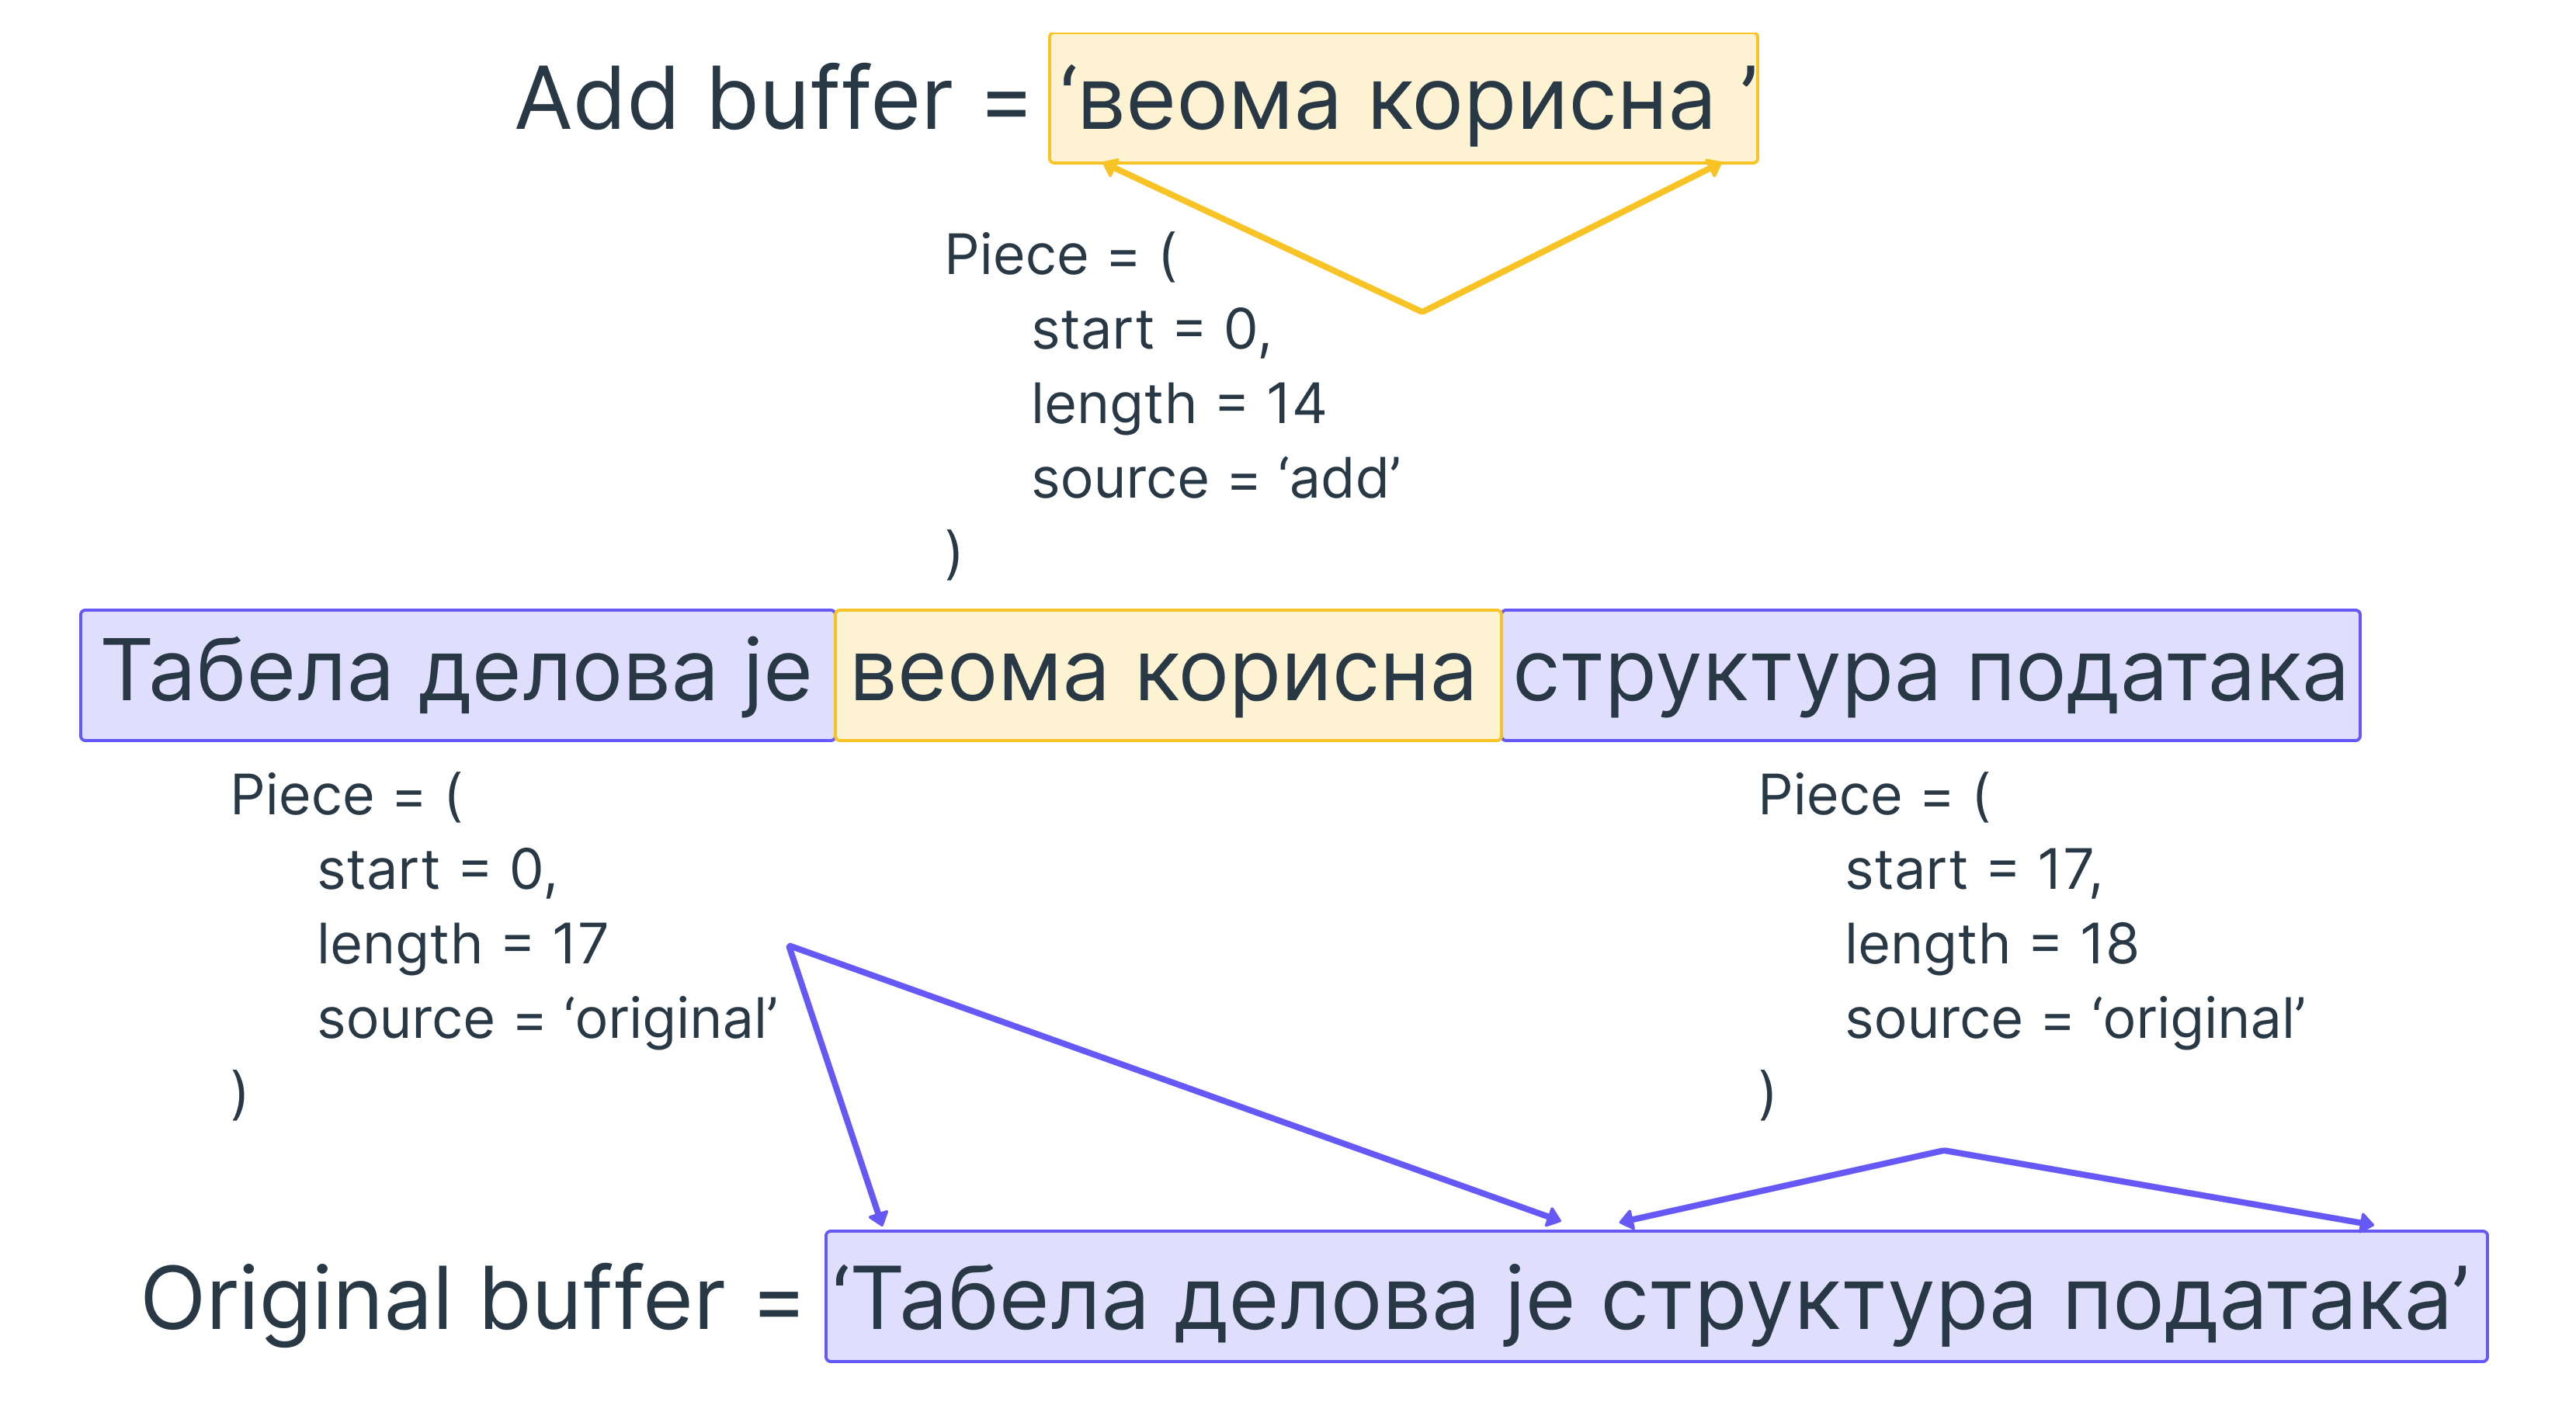
\includegraphics[width=1.0\textwidth]{images/piece_table_1.png}
	\caption{Приказ рада табеле делова}
	\label{fig:piece_table}
\end{figure}

\paragraph{}
По овом механизму где се целокупан текст добија тако што надовезујемо "делове" бафера је сама
структура података добила име. Један од познатијих текст едитора који од 2018. 
користи табелу делова у својој имплементацији је \begin{latinica}\textit{Visual Studio Code}\end{latinica} \cite{VSC}.

\paragraph{}
Сложеност ове операције је \(O(\sum_{i=0}^{m-1} d_i)\) тј једнака је суми
дужина свих дескриптора. Пошто је сума свих дужина једнака дужини укупног текста, онда
се сложеност може једноставније записати као \(O(n)\).

% ------------------------------------------------------------------------------
\chapter{Основне функционалности}
\label{chp:osnovne_funkcionalnosti}

\section{Обрада уноса}
\paragraph{}
Када се користе текст едитори, корисник већину команди задаје преко тастатуре, док се
мањи проценат њих задатаје коришћењем миша. Један од проблема при 
имплементацији текст едитора јесте како исправно обрадити све овакве уносе. 
Пре описа обраде, прво ће бити речи о самим карактерима и њиховим специфичностима. 

\subsection{Карактери}
\paragraph{}
За писање програмског кода најчешће се користи \begin{latinica}\textit{ASCII}\end{latinica} кодирање. \begin{latinica}\textit{ASCII}\end{latinica} табела представља стандард за кодирање
знакова који се користи за представљање текста у рачунарима. Она пресликава знакове
(слова, цифре, интерпункцијске знакове, контролне секвенце, итд.) у бројевне вредности,
омогућавајући на тај начин њихово чување и маниулацију у дигиталним системима. 
\begin{latinica}\textit{ASCII}\end{latinica} стандард користи 7 битова за представљање
сваког карактера, омогућавајући представљање 128 различитих карактера.


\paragraph{}
Немају сви карактери из \begin{latinica}\textit{ASCII}\end{latinica} табеле визуелну
репрезентацију, они који имају вредност у табели од 0 до 31 су тзв. контролни карактери 
(енг. \begin{latinica}\textit{control characters}\end{latinica}) који служе за
слање сигнала за комуникацију са периферним уређајима. Остали карактери, чија је вредност
између 32 и 127, се могу приказивати на излазу и њих називамо штампаним
карактерима (енг. \begin{latinica}\textit{printable characters}\end{latinica}).
На табели \ref{tab:ascii} приказан је њен садржај.

\begin{table}[htbp]
\centering
\setlength{\extrarowheight}{8pt}
\begin{tabularx}{\linewidth}{|X| X | X | X | X | X | X | X | X | X | X | X | X | X | X | X | X|}
	\hline
	& \textbf{0} & \textbf{1} & \textbf{2} & \textbf{3} & \textbf{4} & \textbf{5} & \textbf{6} & \textbf{7} & \textbf{8} & \textbf{9} & \textbf{A} & \textbf{B} & \textbf{C} & \textbf{D} & \textbf{E} & \textbf{F} \\
	\hline
	\textbf{0x} & nul & soh & stx & etx & eot & enq & ack & bel & bs & ht & lf & vt & ff & cr & so & si \\
	\hline
	\textbf{1x} & dle & dc1 & dc2 & dc3 & dc4 & nak & syn & etb & can & em & sub & esc & fs & gs & rs & us \\
	\hline
	\textbf{2x} & sp & ! & \("\) & \(\#\) & \$ & \% & \& & ' & ( & ) & * & \(+\) & , & - & . & / \\
	\hline
	\textbf{3x} & 0 & 1 & 2 & 3 & 4 & 5 & 6 & 7 & 8 & 9 & : & ; & < & = & > & ? \\
	\hline
	\textbf{4x} & @ & A & B & C & D & E & F & G & H & I & J & K & L & M & N & O \\
	\hline
	\textbf{5x} & P & Q & R & S & T & U & V & W & X & Y & Z & [ & \texttt{$\backslash$} & ] & 
	\^{} & \_{} \\
	\hline
	\textbf{6x} & ` & a & b & c & d & e & f & g & h & i & j & k & l & m & n & o \\
	\hline
	\textbf{7x} & p & q & r & s & t & u & v & w & x & y & z & \{ & | & \} & \~{} & del \\
	\hline
\end{tabularx}
\caption{\begin{latinica}\textit{ASCII}\end{latinica} табела.}
\label{tab:ascii}
\end{table}

\subsection{Унос помоћу тастатуре}
\paragraph{}
Уколико корисник притисне неки тастер на тастатури, текст едитор ће га исписати само
ако тастер одговара штампаном карактеру или карактеру за форматирање текста (као што
су \begin{latinica}\textit{Tab}\end{latinica} и \begin{latinica}\textit{Enter}\end{latinica}). Сви остали тастери се игноришу
што омогућава да са неким од њих кодирају друге команде у едитору. 
Поред тога, могуће је комбиновање контролног и штампаног карактера како
би се кодирале додатне команде. Ово се постиже притиском на два или три тастера истовремено. Најчешће се врши комбиновање два тастера, где је први обично \begin{latinica}\textit{Ctrl}\end{latinica}.

\paragraph{}
У имплементацији при раду, обраду ових уноса врши корисничка метода \begin{latinica}\textit{handleKeyboardInput()}\end{latinica} класе
\begin{latinica}\textit{TextEditor}\end{latinica}.
 тако што се стално проверава да ли
је притиснут један или више тастера у датом тренутку и да ли је том комбинацијом 
задата нека специјална команда. Уколико јесте, извршава се одговарајућа команда. Ако
није притиснута ниједна комбинација, гледа се да ли је притиснут неки штампани карактер,
уколико јесте, прослеђује се методи за унос.


\subsection{Унос помоћу миша}
\paragraph{} 
Некада се команде задају и путем миша, али то се своди на померање курсора и означавање
текста. Такође се помоћу менија могу активирати додатне команде и алати.
О курсору и означавању, као и додатним командама биће више речи у наставку рада.
Сигнали који се обрађују су тастер миша који је притиснут (леви, десни и средњи),
позиција курсора миша као и то да ли корисник користи један клик, дупли клик или
држи тастер миша.

\paragraph{}
Имлементација је сложенија него код обраде уноса са тастатуре. Метода
\begin{latinica}\textit{handleMouseInput()}\end{latinica}
класе \begin{latinica}\textit{TextEditor}\end{latinica} обрађује све догађаје
миша. Она се позива периодично и врши проверу да ли је корисник притиснуо леви тастер на мишу, уколико јесте активира се одговарајућа
команда и прослеђује се позиција миша. Такође се проверава да ли је корисник држао
леви тастер и уколико јесте, активира одговарајућу методу и шаље две позиције миша,
у тренутку када је дугме притиснуто и када је отпуштено.


\section{Курсор}
\paragraph{}
Један од основних елемената сваког текст едитора јесте курсор. Његова функција је да
означи место у тексту на којем ће бити извршена следећа измена. Углавном је представљен у 
виду уређеног пара реда и колоне на којој се курсор налази. Иако су у овом раду до сада
измене представљане помоћу индекса неког низа карактера, оваква репрезентација је
интуитивнија и прегледнија за корисника. Оваква репрезентација се користи и
у класи \begin{latinica}\textit{TextCoordinates}\end{latinica} текст едитора.

\begin{minted}{c++}
class TextCoordinates {
	// ...
	public:
	size_t m_row;
	size_t m_col;
};
\end{minted}

\paragraph{}
Такође треба напоменути да у овој репрезентацији обе кординате починњу од
један, а не од нула као код индекса, као и да се вредност колоне може кретати
у целобројном интервалу \([1, d+1]\), где је \(d\) дужина тренутног реда на ком се
курсор налази.

\paragraph{}
Курсор се на већини данашњих рачунара помера позиционирањем миша на жељено место курсора
и притиском на леви тастер или, алтернативно, помоћу стрелица на тастатури. Такође, 
притиском на тастере \begin{latinica}\textit{Home}\end{latinica} и
\begin{latinica}\textit{End}\end{latinica} врши се померање курсора на почетак, односно на крај тренутног реда. У наредном програмском коду
илустроване су неке од метода за померање курсора, док се на слици \ref{fig:cursor}
може видети курсор у текст едитору представљен белом усправном цртом. Такође се
и у статусној линији (на доњем делу едитора) могу видети тренутне координате курсора,
тј. редни број његове врсте и колоне.

\begin{minted}{c++}
class Cursor {
public:
	//...
	void moveRight(size_t times = 1);
	void moveLeft(size_t times = 1);
	void moveUp(size_t times = 1);
	void moveDown(size_t times = 1);
	void moveToBeginning();
	void moveToEnd();
	void moveToEndOfFile();
	//...
};
\end{minted}

\begin{figure}[!ht]
	\centering
	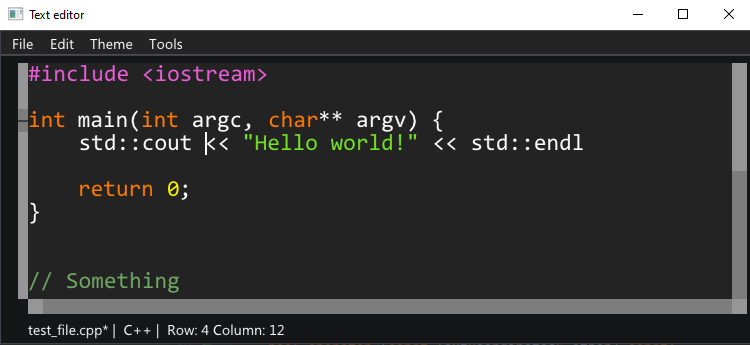
\includegraphics[width=1.0\textwidth]{images/cursor.png}
	\caption{Приказ курсора у текст едитору}
	\label{fig:cursor}
\end{figure}

\section{Операције са појединачним карактерима}

\subsection{Унос}
\paragraph{}
Једна основних функционалности текст едитора је уношење текста карактер
по карактер. Тај унос се врши тако што корисник притиска тастер за одговарајући
штампани карактер и он се уноси на тренутну позицију курсора, тј. испред карактера на ком се налази курсор, уколико није на крају реда, тада се уноси иза последњег карактера. 

\paragraph{}
Унос се имплементира тако што се дохвате координате курсора и прослеђују се 
функцији
\begin{latinica}\textit{textCoordinatesToBufferIndex(TextCoordinates coords)}\end{latinica} 
која преводи уређени пар врсте и колоне у индекс низа карактера. То се постиже на
следећи начин, индекс се на почетку има вредност 0. Пролази се кроз све редове
изнад тренутног, почевши од првог, и на бројач се додаје \(d+1\) (додаје се један да би се урачунао и знак за нови ред), где је \(d\) дужина тог реда. 
Када се стигне до тренутног реда вредност индекса се увећава за вредност колоне умањене за
један. Наредни програмски код илуструје рад ове функције.

\begin{minted}{c++}
size_t LineBuffer::textCoordinatesToBufferIndex
(const TextCoordinates &coords) const {
		
	size_t index = 0;
	
	for (size_t i=0; i<coords.m_row-1; i++)
		index += lineAt(i).size() + 1;
	
	index += (coords.m_col - 1);
	
	return index;
}
\end{minted}

\paragraph{}
Када је добијен индекс низа карактера, он се прослеђује табели делова заједно са  притиснутим карактером и врши се унос и курсор се помера за једно место у десно. 
На примеру функције 
\begin{latinica}\textit{insertCharToPieceTable}\end{latinica} која припада класи
\begin{latinica}\textit{TextBox}\end{latinica} се може видети поступак уметања
карактера у табелу делова.

\begin{minted}{c++}
bool TextBox::insertCharToPieceTable(char c) {
	auto coords = m_cursor->getCoords();
	size_t index = m_lineBuffer->textCoordinatesToBufferIndex(coords);
	return m_pieceTableInstance->getInstance().insertChar(c, index);
}
\end{minted}


\subsection{Брисање}
\paragraph{}
Брисање поједначних карактера се врши тако што корисник позиционира курсор
на жељено место и притисне тастер за брисање карактера. Треба напоменути да 
постоје два тастера за брисање карактера, то су \begin{latinica}\textit{Backspace}\end{latinica}
и \begin{latinica}\textit{Delete}\end{latinica}.
\begin{latinica}\textit{Backspace}\end{latinica} брише карактер лево од курсора,
док \begin{latinica}\textit{Delete}\end{latinica} брише онај на позицији курсора.
После брисања се у првом случају курсор помера за једно место у лево, док у другом
остаје на истој позицији. Брисање је имплементирано на сличан начин као унос.

\paragraph{}
Текст едитор који је имплементиран током рада на овој тези користи две одвојене
методе за обе врсте брисања. То су 
\begin{latinica}\textit{backspace()} \end{latinica} и
\begin{latinica}\textit{deleteChar()} \end{latinica} класе
\begin{latinica}\textit{TextBox} \end{latinica}.

\section{Означавање текста}
\paragraph{}
Означавање текста је функционалност која кориснику пружа могућност означавања
неког непрекидног сегмента текста ради брисања или копирања. Копирање ће бити
објашњено у наставку рада. Означавање текста се најчешће врши помоћу миша, тако што корисник превлачи курсор миша преко дела екрана у коме се налази текст који жели да изабере
и унесе команду за брисање или копирање. Такође се може вршити помоћу тастатуре, тако што
корисник држи тастер \begin{latinica}\textit{Shift}\end{latinica} и стрелицама помера курсор. У овом случају се памти позиција курсора када је притиснут тастер, она ће бити
један крај означеног текста. Други крај ће бити позиција на који је корисник померио
курсор држећи тастер \begin{latinica}\textit{Shift}\end{latinica}.

\paragraph{}
Пре него што буде објашњена импементација, прво ће бити дефинисан поредак између текстуалних координати, о којима је било речи у одељку о курсору. Пошто су координате
представљене уређеним паром реда и колоне,  оне се тако и пореде. Прво се пореде редови, 
па уколико су они једнаки, онда се пореде колоне. У следећем коду илустрована је дефиниција
поређења за операторе \(=\) и \(<\). Симетрични оператори се дефинишу аналогно.

\begin{minted}{c++}
bool TextCoordinates::operator==(const TextCoordinates &other) const {
	return m_row == other.m_row && m_col == other.m_col;
}

bool TextCoordinates::operator<(const TextCoordinates &other) const {
	return (m_row < other.m_row) 
	|| (m_row == other.m_row && m_col < other.m_col);
}
\end{minted}

Oзначавање непрекидног дела текста је у имплементацји при раду представљено помоћу две текстуалне координате. Прва координата представља
локацију на којој почиње текст који је означен, а друга локацију где се завршава. Треба
нагласити да почетак мора бити мањи или једнак од краја. Потребно је, такође, чувати
информацију о томе да ли је означени текст активан. У следећем коду 
илустрован је пример чланских променљивих класе 
\begin{latinica}\textit{Selection}\end{latinica}.

\begin{minted}{c++}
class Selection {
//...
private:
	bool m_active;
	bool m_rectangular;
	TextPosition m_start;
	TextPosition m_end;
};
\end{minted}


\paragraph{}
Када метода \begin{latinica}\textit{handleMouseInput()}\end{latinica} детектује држање
левог тастера, она прослеђује две позиције миша методи \begin{latinica}\textit{setMouseSelection()}\end{latinica} класе
\begin{latinica}\textit{TextBox}\end{latinica}. Онда она на основу те две позиције
рачуна на које текстуалне координате оне показују и додељује мању од вредности координати
која означава почетак, а већу координати која означава крај. 
На крају се означени текст обележава као активан.

\paragraph{}
Уколико је означени текст активан и корисник кликне било где на текстуално поље едитора,
он се деактивира. Такође се може деактивирати притиском на стрелице за померање
курсора. При притиску на тастере за брисање док је означени текст активан, сав означени
текст се брише. Исто важи и за операције исецања
(енг. \begin{latinica}\textit{cut}\end{latinica}) и налепљивања
(енг. \begin{latinica}\textit{paste}\end{latinica}). Деактивирање озанченог текста
се имплементира тако што се чланска променљива 
\begin{latinica}\textit{m\_active}\end{latinica} постави на вредност
\begin{latinica}\textit{false}\end{latinica}.

\paragraph{}
Притиском на комбинацију тастера \begin{latinica}\textit{Shift}\end{latinica} и
\begin{latinica}\textit{Home}\end{latinica} се почетак означавања поставља на почетак реда,
а крај на тренутну позицију курсора, док се притиском на тастере 
\begin{latinica}\textit{Shift}\end{latinica} и \begin{latinica}\textit{End}\end{latinica}
почетак означавања поставља на позицију курсора, а крај на последњу колону у реду.
Притиском на комбинацију тастера \begin{latinica}\textit{Ctrl}\end{latinica} и
\begin{latinica}\textit{A}\end{latinica} означава се читав текст. На слици 
\ref{fig:selection} се може видети пример означавања, где је означени део текста
уоквирен правоугаоником другачије боје од позадине.

\begin{figure}[!ht]
	\centering
	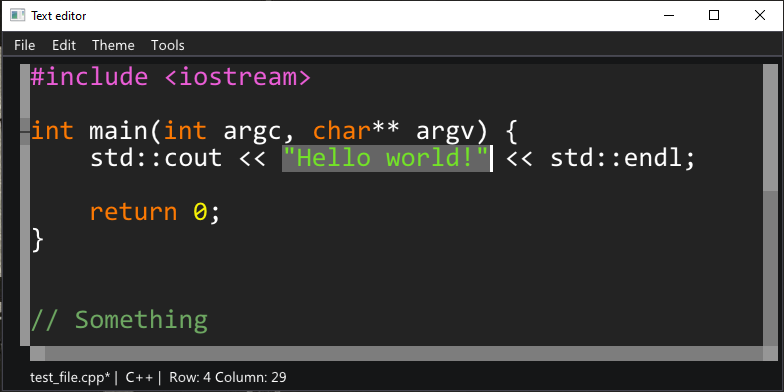
\includegraphics[width=1.0\textwidth]{images/selection.png}
	\caption{Приказ означавања у текст едитору}
	\label{fig:selection}
\end{figure}

\section{Управљање текстуалним датотекама}
\paragraph{}
Сврха текст едитора јесте мењање текстуалних датотека или писање нових. 
Да би то било могуће, потребно је обезбедити кориснику могућности креирања нових датотека,
као и отварање постојећих. Такође је потребно омогућити чување измена које корисник
прави као и могућност избора локације где ће датотека бити сачувана.  У наредним
пододељцима биће обрађене те функционалности. 

\subsection{Чување датотека}
\paragraph{}
Корисник може сачувати тренутни садржај едитора у датотеку притиском на дугме 
\begin{latinica}\textit{Save}\end{latinica} у менију или комбинацијом
тастера \begin{latinica}\textit{Ctrl}\end{latinica} и
\begin{latinica}\textit{S}\end{latinica}. Тренутни садржај се чува на 
жељену локацију и уколико није дефинисана, тражи се од корисника
да је унесе. Такође је дозвољено и чување тренутне датотеке на нову локацију
притиском на дугме \begin{latinica}\textit{Save as}\end{latinica} у менију, где
је поступак исти као са недефинисаном путањом.

\paragraph{}
Чување датотека у имплементацији при раду извршава метода
\begin{latinica}\textit{save()}\end{latinica} класе
\begin{latinica}\textit{TextEditor}\end{latinica} и може се видети у наредном
програмском коду.

\begin{minted}{c++}
void TextEditor::save() {
	if (m_activeTextBox->getFile() == nullptr)
		saveAs();
	else {
		m_activeTextBox->save();
		m_inactiveTextBox->save();
	}
}
\end{minted}

\paragraph{}
За недефинисану путању позива се метода
\begin{latinica}\textit{saveAs()}\end{latinica}, док се у супротном
зове метода \begin{latinica}\textit{save()}\end{latinica} класе
\begin{latinica}\textit{TextBox}\end{latinica} која уписује садржај
едитора преко старог садржаја датотеке на задатој путањи. Следећи програмски к\^{о}д
илуструје методу \begin{latinica}\textit{saveAs()}\end{latinica}.

\begin{minted}{c++}
void TextEditor::saveAs() {
	auto path = saveFileDialog();
	
	if (!path.empty()) {
		if (path.find_last_of('.') == std::string::npos)
		path += ".txt";
		m_activeTextBox->saveAs(path);
		m_inactiveTextBox->saveAs(path);
	}
}
\end{minted}

\paragraph{}
Она отвара дијалог где корисник треба да изабере локацију где ће бити сачувана
датотека и враћа путању. Уколико није дефинисана, екстензија 
(енг. \begin{latinica}\textit{extension}\end{latinica}) датотеке биће
постављена на обичну текстуалну датотеку (\begin{latinica}\textit{.txt}\end{latinica}).
Затим се позива истоимена метода класе \begin{latinica}\textit{TextBox}\end{latinica} која
поставља нову путању и уписује садржај едитора на дату локацију.

\paragraph{}
Да би се водила евиденција о изменама у тренутној датотеци користи
се индикатор који се назива прљави бит (енг \begin{latinica}\textit{dirty bit}\end{latinica}). Он се активира уколико постоје неке измене које нису сачуване. 
Када корисник отвара датотеку, прљави бит је неактиван.
Сваком променом текста активира се прљави бит, док се сваким
чувањем деактивира. Он је обично представљен карактером звездице поред
имена датотеке која је отворена.

\subsection{Отварање нове датотеке}
\paragraph{}
Корисник може отворити нову датотеку на дугме 
\begin{latinica}\textit{New file}\end{latinica} у менију или комбинацијом тастера
\begin{latinica}\textit{Ctrl}\end{latinica} и
\begin{latinica}\textit{N}\end{latinica}. Када корисник покрене ову акцију,
тренутни фајл се затвара и уколико је активан прљави бит, едитор отвара
дијалог где корисника пита да ли жели да сачува измене. Затим се садржај
текстуалног поља као и табеле делова се ресетује и курсор се поставља на почетак.

\paragraph{}
У имплементацији при раду за ову функционалност задужена је метода
\begin{latinica}\textit{newFile()}\end{latinica} класе
\begin{latinica}\textit{TextEditor}\end{latinica}. Она проверава да ли је фајл
сачуван и позива методу
\begin{latinica}\textit{handleFileNotSaved()}\end{latinica} 
уколико није. Затим позива истоимену методу класе \begin{latinica}\textit{TextBox}\end{latinica} која ресетује свој садржај.
У наредном примеру кода се може видети описана метода.

\begin{minted}{c++}
void TextEditor::newFile() {
	auto id = handleFileNotSaved();
	if (id == IDCANCEL)
	return;
	
	m_activeTextBox->newFile();
	if (m_splitScreen)
	m_inactiveTextBox->setFile(m_activeTextBox->getFile());
}
\end{minted}

\subsection{Отварање постојеће датотеке}
\paragraph{}
Уколико корисник жели да отвори постојећу датотеку он може то учинити притиском
на дугме \begin{latinica}\textit{Open}\end{latinica} у менију или комбинацијом
тастера \begin{latinica}\textit{Ctrl}\end{latinica} и \begin{latinica}\textit{O}\end{latinica}. Када покрене ову команду, корисник
бира датотеку коју жели и она се отвара у тескст едтиору. Ову функционалност
имплементира метода \begin{latinica}\textit{open()}\end{latinica} класе
\begin{latinica}\textit{TextEditor}\end{latinica}. Она је приказана
на следећем примеру кода.

\begin{minted}{c++}
void TextEditor::open() {
	auto id = handleFileNotSaved();
	if (id == IDCANCEL)
	return;
	
	auto path = openFileDialog();
	
	if (!path.empty()) {
		m_activeTextBox->open(path);
		m_inactiveTextBox->open(path);
	}
}
\end{minted}

\paragraph{}
Прво се проверава прљави бит, и уколико је активан отвара дијалог за чување помоћу
функције \begin{latinica}\textit{handleFileNotSaved()}\end{latinica}. Затим се 
отвара дијалог за избор датотеке помоћу функције
\begin{latinica}\textit{openFileDialog()}\end{latinica}  и враћа се изабрана
путања. На крају се позива истоимена меотда класе
\begin{latinica}\textit{TextBox}\end{latinica} и отвара се датотека и њен садржај
се учитава у едитор.

\section{Исецање, Копирање и налепљивање}
\paragraph{}
Исецање (енг. \begin{latinica}\textit{cut}\end{latinica}), копирање
(енг. \begin{latinica}\textit{copy}\end{latinica}) и налепљивање
(енг. \begin{latinica}\textit{paste}\end{latinica}) су операције
које раде са меморијском таблом 
(енг. \begin{latinica}\textit{clipboard}\end{latinica}), која је део меморије
у оперативним системима који је резервисан за привремено чување као и пренос
података између више програма или унутар једног. Ти подаци могу бити текст,
слике, датотеке, итд. Овај одељак ће се бавити преносом текста. Табла функционише
тако што по потреби можемо писати у њу или читати из ње. Обично се у једном
тренутку може налазити само један податак у табли.

\paragraph{}
Ове три операције представљају једне од највећих предности коришћења текст едитора,
јер омогућавају копирање великих делова текста и њихово премештање. Код писања к\^{о}да,
ово посебно долази до изражаја јер често постоје делови к\^{o}да који се појављују више пута и ова функционалност штеди доста времена програмерима.

\subsection{Исецање}
\paragraph{}
Исецање (енг. \begin{latinica}\textit{cut}\end{latinica}) је операција која
копира тренутно означени текст и уписује га у меморијску таблу и затим га
брише из текста. У наредном примеру к\^{о}да дата је њена имплементација.

\begin{minted}{c++}
void TextBox::cut() {
	if (m_selection->isActive()) {
		copySelectionToClipboard();
		deleteSelection();
	}
}
\end{minted}

\paragraph{}
Прво се проверава да ли је неки текст означен, ако јесте копира се њен садржај у
таблу, и затим се брише означени текст. У следећем к\^{о}ду дата је имплеметнација
методе \begin{latinica}\textit{copySelectionToClipboard()}\end{latinica}.

\begin{minted}{c++}
void TextBox::copySelectionToClipboard() {
	auto selectionText = m_selection->getSelectionText();
	ImGui::SetClipboardText(selectionText.c_str());
}
\end{minted}

\paragraph{}
Метода је врло једноставна, дохвата се означени текст и поставља се као
текст меморијске табле.

\subsection{Копирање}
\paragraph{}
Копирање (енг. \begin{latinica}\textit{copy}\end{latinica}) уписује означени
текст у меморијску таблу. За разлику од исецања текст се не брише. Следећи к\^{о}д
садржи њену имплементацију.

\begin{minted}{c++}
void TextBox::copy() {
	if (m_selection->isActive()) {
		copySelectionToClipboard();
	}
}
\end{minted}

\subsection{Налепљивање}
\paragraph{}
Налепљивање (енг. \begin{latinica}\textit{paste}\end{latinica}) уписује текст из
меморијске табле на тренутну позицију курсора. У наредном к\^{о}ду садржана је њена
имплементација.

\begin{minted}{c++}
void TextBox::paste() {
	auto text = std::string(ImGui::GetClipboardText());
	if (!text.empty())
	enterText(text);
}
\end{minted}
% ------------------------------------------------------------------------------


% ------------------------------------------------------------------------------
\chapter{Напредне функционалности}
% ------------------------------------------------------------------------------
\section{Враћање уназад и унапред}
\paragraph{}
Враћање уназад (енг. \begin{latinica}\textit{undo}\end{latinica}) је функционалност
која поништава измене у тексту и враћа га у пређашње стање. Са друге стране,
враћање унапред (енг. \begin{latinica}\textit{redo}\end{latinica}) поставља текст у стање пре поништавања (уколико је поништена нека акција). Дата
функционалност пружа могућност кориснику да се врати у неко прошло стање
уколико је направљена грешка или обрисан неки битан део текста.
Даље објашњење ове функционалности биће илустровано кроз к\^{о}д текст едитора 
имплемнтираног при раду на овој тези.

\paragraph{}
Да би се дефинисало поништавање акција и њихово враћање, прво се морају дефинисати саме акције. Свака измена над текстом у табели делова чини једну
акцију. Оне се састоје од ознаке да ли се ради о уметању или брисању, индекса
на коме почиње измена и низа дескриптора промене. Овај низ садржи редом, 
с лева  на десно, дескрипторе делова који заједно чине додати или обрисани текст.
У следећем програмском коду илустроване су чланске променљиве класе 
\begin{latinica}\textit{ActionDescriptor}\end{latinica}.

\begin{minted}{c++}
class ActionDescriptor {
	//...
	private:
	ActionType m_actionType;
	std::vector<PieceDescriptor*> m_descriptors;
	size_t m_index;
};
\end{minted}


\paragraph{}
Код уметања текста у табелу делова, акција се дефинише тако што јој
се додели одговарајућа ознака, индекс на коме је извршено уметање и
један дескриптор који садржи додати текст на крају бафера за додавање.

\paragraph{}
Код брисања се индекс поставља на почетак обрисаног текста, док је низ
дескриптора компликованији него код уметања. Пошто се код брисања може
обрисати више дескриптора, онда и низ може садржати више елемената. Ако
се брише цео дескриптор, онда се он цео додаје у низ. Уколико се дескриптор
скраћује са почетка или краја, онда се прави нови дескриптор који показује
на обрисани део и додаје се у низ. Исто важи и за случај када се уклања
текст из средине једног дескриптора, тј. прави се дескриптор који показује
на средину која је обрисана.

\paragraph{}
Када је познато шта представља једна акција, једноставније је дефинисати како 
се поништава. Поништавање се врши помоћу стека за враћање уназад 
(енг. \begin{latinica}\textit{undo stack}\end{latinica}) који чува у себи
акције. Сваки пут када се изврши нека акција, додаје се на врх стека. Враћање
уназад се врши тако што се дохвати акција са врха стека, провери се која је 
операција вршена и затим се изврши супротна акција. После тога, дескриптору
акције се додељује супротна ознака и додаје се у стек за враћање унапред
(енг. \begin{latinica}\textit{redo stack}\end{latinica}).

\paragraph{}
Поставља се питање шта чини супротну акцију? Супротна акција ће бити дефинисана
одвојено за случај уметања и случај брисања текста. Код уметања текста, иде се
редом кроз листу дескриптора и сабирају се њихове дужине. Нека је сума
дужина означена са \(d\), а почетни индекс акције са \(p\), онда се брише
текст из табеле који припада целобројном интервалу \([p, p+d)\).

\paragraph{}
Код брисања се дефинише индекс за уметање који има вредност почетног индекса акције. Затим се додају редом дескриптори на место индекса за уметање и после сваког уметања се повећава индекс за дужину дескриптора. У наредном програмском
коду илустровано је извршавање обрнуте операције са врха стека и њено постављање
на други стек.

\begin{minted}{c++}
void PieceTable::reverseOperation
(std::stack<ActionDescriptor*>& stack, 
 std::stack<ActionDescriptor*>& reverseStack) {
	
	if (stack.empty())
		return;
	
	auto action = stack.top();
	stack.pop();
	
	auto actionType = action->getActionType();
	auto descriptors = action->getDescriptors();
	auto index = action->getIndex();
	size_t totalLength = 0;
	
	if (actionType == ActionType::Insert) {
		totalLength = std::accumulate(
			descriptors.begin(), 
			descriptors.end(), 
			(size_t)0,
			[](size_t acc, PieceDescriptor* descriptor) 
				{ return  acc + descriptor->getLength(); }
		);
		
		deleteText(index, index+totalLength, true);
	} else {
		for (size_t i=0; i<descriptors.size(); ++i) {
			auto source = descriptors[i]->getSource();
			auto start = descriptors[i]->getStart();
			auto length = descriptors[i]->getLength();
			
			insert(source, start, length, index+totalLength, true);
			totalLength += length;
		}
	}
	
	auto oppositeActionType = 
		ActionDescriptor::getOppositeActionType(actionType);
		
	action->setActionType(oppositeActionType);
	
	reverseStack.push(action);
}
\end{minted}

\paragraph{}
Враћање унапред се врши потпуно идентично, само се акција дохвата
са стека за враћање унапред и супротна акција се ставља на стек за враћање
уназад. Да се видети да су ове операције потпуно симетричне, с тим да се након 
извршавања неке акције она додаје само на стек за враћање уназад, док се елементи могу додати на стек за враћање унапред само путем враћања уназад. У следећем
коду је илустрована симетричност ових операција.

\begin{minted}{c++}
void PieceTable::undo() {
	reverseOperation(m_undoStack, m_redoStack);
}

void PieceTable::redo() {
	reverseOperation(m_redoStack, m_undoStack);
}
\end{minted}

\paragraph{}
Када се користи ова функционалност у текст едиторима може се приметити да 
враћање уназад и унапред обично враћају целе делове текста, а не појединачне
карактере. Таква имплементација је интуитивна из угла корисника јер је најчешће
потребно поништити веће делове текста уместо један карактер.

\paragraph{}
Овакав ефекат се постиже тако што се уводе два бафера, један за уметање и један
за брисање. Бафер за уметање садржи све карактере који су тренутно унесени у 
непрекидном низу. Када се низ прекине, било уносом који се не наставља на тренутни
низ, било брисањем неког дела текста, бафер се празни и цео његов садржај се уноси
у табелу делова и акција се ставља на стек за враћање уназад. 
Бафер за брисање ради по истом принципу као и онај за уметање, само се код њега
чува почетни и крајњи индекс обрисаног дела текста.

\paragraph{}
Све време када бафери нису празни, табела делова даје привид да су све досадашње
измене унете у њу, док се у позадини оне тек уносе по пражњењу бафера. У надредна
два примера кода илустровано је редом: чланске променљиве класе \begin{latinica}
\textit{InsertBuffer}\end{latinica}, уношење појединачног карактера у текст.

\begin{minted}{c++}
class InsertBuffer {
	//...
	private:
	bool m_flushed;
	size_t m_startIndex;
	size_t m_endIndex;
	std::string m_content;
};
\end{minted}

\begin{minted}{c++}
bool PieceTable::insertChar(char c, size_t index) {
	if (index != m_insertBuffer->getEndIndex()) {
		flushInsertBuffer();
	}
	
	bool result = false;
	
	if (m_insertBuffer->isFlushed()) {
		m_insertBuffer->setStartIndex(index);
		m_insertBuffer->setEndIndex(index);
		m_insertBuffer->setFlushed(false);
		result = true;
	}
	
	m_insertBuffer->appendToContent(c);
	return  result;
}
\end{minted}

\paragraph{}
За крај треба напоменути да је овакву имплементацију враћања уназад и унапред
омогућено коришћењем табеле делова. Пошто се текст не брише из бафера могуће
је једноставније враћање обрисаних делова текста. Имплементација помоћу других
структура била би значајно сложенија.

\section{Назначавање синтаксе}

\paragraph{}
Назначавање синтаксе (енг. \begin{latinica}\textit{syntax highlighting}\end{latinica})
је напредна функционалност која омогућава кориснику бољу прегледност при писању
програмског кода тако што се различити токени као што су ниске, бројеви, кључне речи, коментари, имена функција итд. назначавају различитим бојама.  Овим се постиже боља читљивост кода јер корисник лакше разазнаје различите целине у коду.

\paragraph{}
У имплементацији при раду токени који се назначавају су кључне речи, ниске, бројеви, претпроцесорске директиве и коментари (једнолинијски и вишелинијски).
Подржани програмски језици за назначавање су
\begin{latinica}\textit{C++}\end{latinica}, \begin{latinica}\textit{C}\end{latinica},
\begin{latinica}\textit{C\#}\end{latinica} и \begin{latinica}\textit{Java}\end{latinica}. За сваки језик се чувају
информације о њему као што су да ли има претпроцесорске директиве, како
се отварају једнолинијски коментари, како се отварају и затварају вишелинијски
коментари и скуп кључних речи.У наредном примеру кода илустроване су те
информације у класи \begin{latinica}\textit{Language}\end{latinica}.

\begin{minted}{c++}
class Language {
//...
private:
	std::set<std::string> m_keywords;
	std::string m_singleLineCommentStart;
	std::string m_multiLineCommentStart;
	std::string m_multiLineCommentEnd;
	std::string m_name;
	bool m_preprocessor;
};
\end{minted}

\paragraph{}
Такође се чува информација о томе за који програмски језик је укључено
назначавање. Он се одређује на основу екстензије отвореног фајла, уколико
екстензија није подржана поставља се мод за обичан текст који не примењује
никакво назначавање.

\paragraph{}
Ова функционалност се реализује тако што чувамо за сваки карактер у тексту његову тренутну боју. Чува се дводимензиона листа где \(j\)-ти елемент \(i\)-те
листе одговара \(j\)-том карактеру \(i\)-те линије. Ова тзв. "мапа боја" се
ажурира тако што се за различите категорије токена врше провере проласком
кроз текст и уписивањем одговарајућих вредности у мапу.

\paragraph{}
За претпроцесорске директиве се проверава само да ли линија почиње карактером
\textit{\#} и уколико је услов испуњен цела линија се назначава одговарајућом бојом.

\paragraph{}
За једнолинијске коментаре у свакој линији се тражи ниска \textit{//} и уколико
је пронађена, она и сав текст десно од ње у линији назначава се бојом за
коментаре.

\paragraph{}
За ниске се користи претрага помоћу регуларних израза и уколико је пронађено
поклапање, поклопљени текст се назначава бојом за ниске. У наредном програмском
коду приказан је регуларни израз који се користи за претрагу.

\begin{minted}{c++}
const std::regex TextHighlighter::m_stringRegex = std::regex(
	R"((['"])((\\\1|.)*?)\1)"
);
\end{minted}

\paragraph{}
За бројеве и кључне речи користи се парсер који разбија линију на токене и за 
сваки токен се проверава да ли је симбол, уколико јесте проверава се да ли је 
садржан у скупу кључних речи. Ако је и овај услов испуњен, токен се означава 
као кључна реч. У супротном се проверава да ли је токен број и уколико јесте
назначава се правилном бојом. У наредном примеру кода илустрована је функција
која у једној линији тражи све горенаведене токене и враћа исправно обојену
мапу за ту линију.

\begin{minted}{c++}
std::vector<ThemeColor> TextHighlighter::getColorMap
	(std::string& line, LanguageMode mode) {
		
	std::vector<ThemeColor> colorMap(line.size(), ThemeColor::TextColor);
	
	if (LanguageManager::getLanguage(mode)->isPreprocessor())
	searchForPreprocessorCommands(line, colorMap);
	
	searchRegex(line, colorMap, m_stringRegex, ThemeColor::StringColor);
	searchForSingleLineComment(line, colorMap, mode);
	searchForKeywordsAndNumbers(line, colorMap, mode);
	
	return colorMap;
}
\end{minted}

\paragraph{}
На крају се траже вишелинијски коментари. У свакој линији се тражи отварајућа
ознака која је једнака нисци \textit{/*} и када се наиђе на њу пролази се кроз
текст док се не пронађе затварајућа ознака која је једнака нисци \textit{*/}.
Тада се обе ознаке и текст између њих боје у одговарајућу боју и потом се поново
понавља процес тражења отварајуће ознаке. Уколико се при проналажењу неке отварајуће
ознаке не пронађе затварајућа онда се текст боји од почетка отварања коментара па до краја самог текста.

\paragraph{}
Треба нагласити да постоји приоритет између различитих токена тј.
уколико неки део текста може бити обојен са више боја треба изабрати
само једну. Унутар коментара и ниски ништа нема приоритет над њима,
код претпроцесорских директива једино коментари имају већи приоритет,
док бројеви и кључне речи имају најнижи приоритет.
На слици \ref{fig:text_highlighting} илустровано је назначавање
једног програмског кода.  Претпроцесорске директиве обојене су у розе,
коментари тамно зеленом бојом, ниске су обојене у светло зелено, бројеви у
жуто, док су кључне речи обојене наранџасто.

\begin{figure}[!ht]
	\centering
	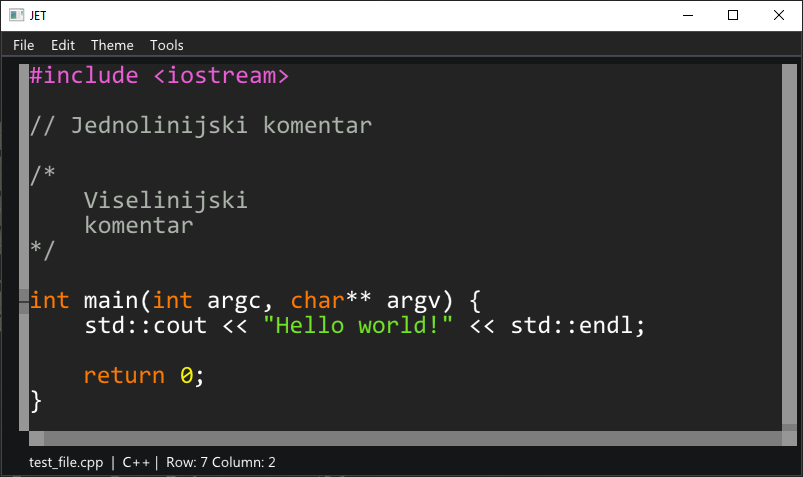
\includegraphics[width=1.0\textwidth]{images/text_highlighting.png}
	\caption{Приказ назначавања програмског кода}
	\label{fig:text_highlighting}
\end{figure}


\section{Правоугаоно означавање}

\paragraph{}
У општем случају, означени текст представља непрекидни део текста
између почетне и крајње координате. Међутим, правоугаоно означавање
омогућава да се изабере само онај текст који је унутар правоугаоника
који чине почетна и крајња координата. 

\paragraph{}
То се постиже тако што се додаје индикатор који нам говори да ли
је означавање обично или је правоугаоно. При дохватању означеног
текста, прво проверава вредност индикатора. Уколико се ради о обичном
означавању, две координате се преводе у индексе и дохвата се текст између
њих. Уколико је се ради о правоугаоном означавању, онда се за сваку линију
почевши од линије почетне координате па до крајње, дохвата текст између колона
почетне и крајње координате. У наредном програмском коду је илустрована ова
функционалност.

\begin{minted}{c++}
std::string Selection::getSelectionText() {
	std::string result;
	TextCoordinates it = m_start.getCoords();
	
	// Dohvata se pokazivač na početnu liniju
	std::string* line = &m_lineBuffer->lineAt(it.m_row-1);
	
	// Iteriranje dok se ne stigne do kraja selekcije
	while (it < m_end.getCoords()) {
		// Ako je kolona van granica, ide se na narednu liniju
		if (it.m_col > line->size() 
		|| (m_rectangular && it.m_col >= m_end.getCoords().m_col)) {
			result += '\n';
			it.m_row += 1;
			it.m_col = m_rectangular ? m_start.getCoords().m_col : 1;
			
			line = &m_lineBuffer->lineAt(it.m_row-1);
		} else {
			if (!line->empty())
			result.push_back(line->at(it.m_col-1));
			
			it.m_col += 1;
		}
	}
	
	return result;
}
\end{minted}

\paragraph{}
Ова функционалност омогућава једноставно дохватање испрекиданих делова
текста као што су колоне у текстуалним табелама као и делове кода без дохватања
карактера за назубљивање. На слици \ref{fig:rectangular_selection} илустровано
је правоугаоно означавање где је означен унутрашњи део звездица.

\begin{figure}[!ht]
	\centering
	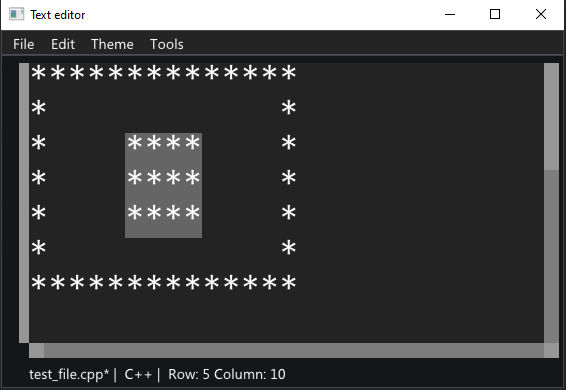
\includegraphics[width=1.0\textwidth]{images/rectangular_selection.png}
	\caption{Приказ правоугаоног означавања}
	\label{fig:rectangular_selection}
\end{figure}

\section{Подела екрана}

\paragraph{}
Дељење екрана пружа кориснику могућност да има два текстуална поља
којима може мењати исти датотеку истовремено. Корисник укључује и искључује овај
режим преко менија у зависности од потребе. Ова функционалност је корисна
у случајевима када текстуална датотека садржи велики број линија и корисник
може лакше да мења два удаљена места у тексту без сталног пребацивања
између њих.

\paragraph{}
У имплементацији при раду је ова функционалност остварена тако што
се цртају два објекта класе \begin{latinica}\textit{TextBox}\end{latinica}
који деле показивач на исту табелу делова. Осим табеле, све између
два текстуална поља је одвојено.
На слици \ref{fig:split_screen} је илустровано дељење екрана за једну
датотеку.

\begin{figure}[!ht]
	\centering
	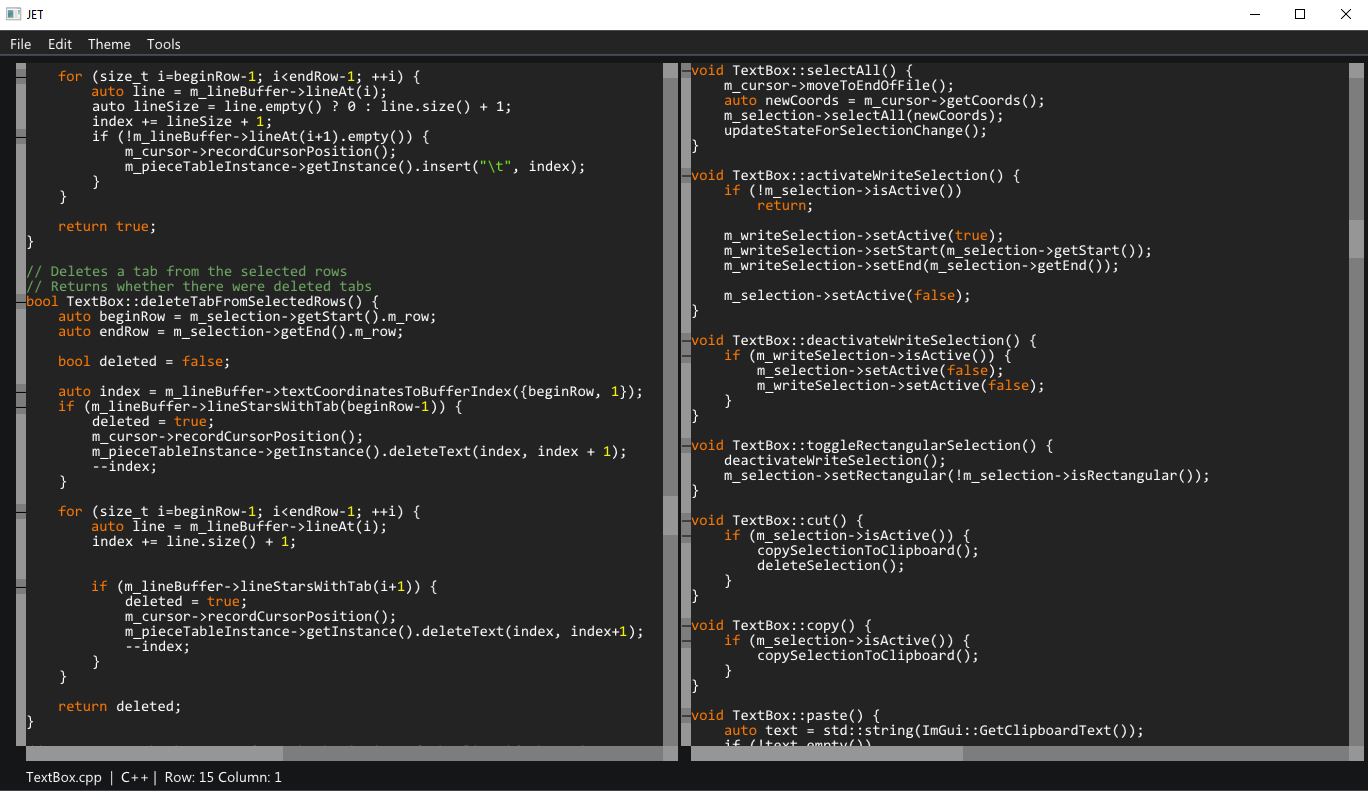
\includegraphics[width=1.0\textwidth]{images/split_screen.png}
	\caption{Приказ поделе екрана}
	\label{fig:split_screen}
\end{figure}


\section{Сужавање простора за измену}

\paragraph{}
Ова функционалност омогућава да се место на коме корисник жели да изврши
измене сузи на неки произвољни опсег текста. Корисник означава неки део текста,
активира ову функционалност из менија и од тада је могуће вршити измене само
унутар означеног дела. Корисник у сваком тренутку може искључити сужавање, враћајући се у уобичајени режим. Ова функционалност може бити корисна у
случајевима када је потребно мењати мање делова кода без нарушавања околне
структуре. Пример овакве измене може бити промена имена функције или променљиве.


\paragraph{}
У имплементацији при раду ова функционалност је остварена тако што се при
активирању овог режима памте почетак и крај означеног текста уколико је активно
неко означавање, ако није означен текст није могуће активирати овај режим.
Затим се кретање курсора и даље означавање текста ограничава на сужени део
за измене. Такође се део за измене сужава или проширује у зависности од тога
да ли се брише или додаје текст у суженом простору. На слици
\ref{fig:edit_narrowing} илустровано је сужавање дела за измену на име главне
функције.

\begin{figure}[!ht]
	\centering
	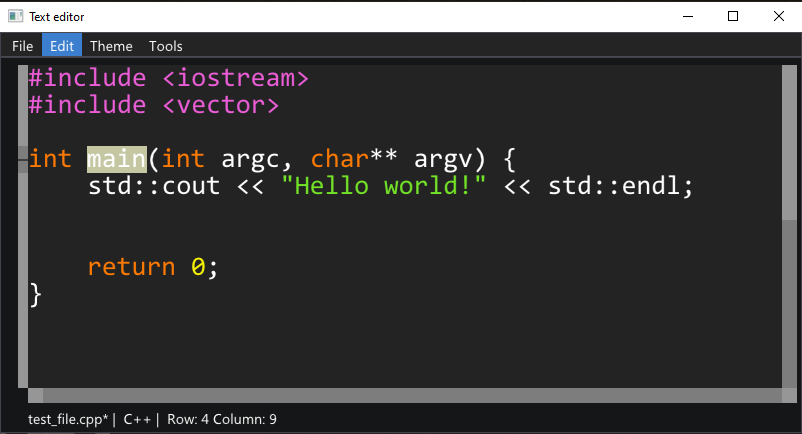
\includegraphics[width=1.0\textwidth]{images/edit_narrowing.png}
	\caption{Приказ сужавања дела за измену}
	\label{fig:edit_narrowing}
\end{figure}


\section{Чување исечака кода}

\paragraph{}
Као што име одељка каже, функционалност омогућава кориснику да сачува
исечке кода које често користи при писању програмског кода. Сваки исечак састоји се од имена и његовог садржаја. Ова функционалност се користи тако
што корисник отвара мени за исечке где му се приказују сви исечци. Када
одабере жељени исечак корисник може прекопирати његов текст или га обрисати у зависности од потребе. Корисник може додати нови исечак означавањем жељеног текста и одабиром одговарајуће акције из менија, 
затим корисник уноси име новог исечка и уколико не постоји исечак
са истим именом, додаје се у колекцију. 

\paragraph{}
У имплементацији при раду, исечци се чувају у датотекама које се по
потреби дохватају и њихов садржај се исписује у менију. Овај мени
је илустрован на слици \ref{fig:code_snippets}.

\begin{figure}[!ht]
	\centering
	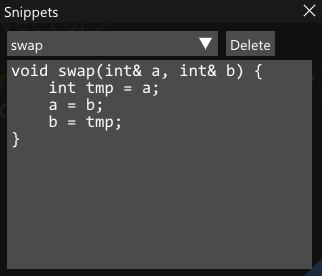
\includegraphics[width=0.7\textwidth]{images/code_snippets.png}
	\caption{Приказ менија за исечке}
	\label{fig:code_snippets}
\end{figure} 
% ------------------------------------------------------------------------------
% Literatura
% ------------------------------------------------------------------------------
\literatura

% ==============================================================================
% Završni deo teze i prilozi
\backmatter
% ==============================================================================

% ------------------------------------------------------------------------------
% Biografija kandidata
\begin{biografija}
\textbf{Бојан Барџић} је рођен 5. априла 1999. године у Призрену. Основне студије
је завршио на Математичком факултету у Београду, на смеру информатика 2022. године
са просечном оценом 8.64. Тренутно је студент мастер студија на истом факултету.
\end{biografija}
% ------------------------------------------------------------------------------

\end{document} 